% AAMAS 2013 Manuscript

% This file should be compiled with "aamas2013.cls" 
% ----------------------------------------------------------------------
% REMEMBER: After having produced the .bbl file,
% and prior to final submission, you *NEED* to 'insert'
% your .bbl file into your source .tex file so as to provide
% ONE 'self-contained' source file.
% ----------------------------------------------------------------------

%%%%%%%%%%%%%%%%%%%%%%%%%%%%%%%%%%%%%%%%%%%%%%%%%%%%%%%%%%%%%%%%%%%%%%%%%%%%%%
% STYLE NOTES
%
% TENSE AND VOICE
% * Actual experimental events
% 	We wrote descriptions of actual experimental events using past tense, in 
%	active voice, as the first person plural.
%
% * All other contexts
%	We write all other text using present tense, in active voices, as the
%	the first person plural.  
%
% CONVENTIONS
% flapping-wing, small-scale, lightweight, MAV
%
%%%%%%%%%%%%%%%%%%%%%%%%%%%%%%%%%%%%%%%%%%%%%%%%%%%%%%%%%%%%%%%%%%%%%%%%%%%%%%
% SETUP
\documentclass{aamas2013}

%----------------------------------------------------------------------------%
% PACKAGES
\usepackage{color}
\usepackage[pdftex]{hyperref}
\usepackage{amsmath}
\usepackage{amssymb}
\providecommand{\norm}[1]{\lVert#1\rVert}

%----------------------------------------------------------------------------%
% METADATA
\def \papertitle{Cooperative Control and Modeling for Narrow Passage Traversal with an 
Ornithopter MAV and Lightweight Ground Station}
\def \paperkeywords{AAMAS proceedings, multiagent systems, cooperative control, 
particle filter, micro air vehicle, ground station, visual servoing, pose 
estimation, flapping wing, ornithopter, biomimetic}
\def \paperterms{Algorithms, Performance, Design, Experimentation}
%\def \paperauthors{Ryan C. Julian, Cameron J. Rose, Humphrey Hu, and Ronald S. Fearing}
\def \paperauthors{Paper 580}

% Set title
\title{\papertitle}

% PDF bookmarks
\definecolor{linkCol}{gray}{0.25}
\hypersetup{
    pdftitle={\papertitle},
    pdfauthor={\paperauthors},
    pdfsubject={\paperterms},
    pdfkeywords={\paperkeywords},
    pdfpagemode=UseOutlines, bookmarksopen, bookmarksnumbered,
    colorlinks, linkcolor=linkCol, citecolor=linkCol, urlcolor=linkCol
}

%----------------------------------------------------------------------------%
% pdfLatex clean-up 
\pdfpagewidth=8.5truein
\pdfpageheight=11truein

\begin{document}

%%%%%%%%%%%%%%%%%%%%%%%%%%%%%%%%%%%%%%%%%%%%%%%%%%%%%%%%%%%%%%%%%%%%%%%%%%%%%%
% AUTHORS

%% Paper number instead of authors
%\numberofauthors{1}
%\author{
%\alignauthor Paper  580
%}

\numberofauthors{4}
\author{
\alignauthor Ryan C. Julian\\
       \affaddr{Department of EECS}\\
       \affaddr{Univ. of California, Berkeley}\\
       \affaddr{Berkeley, CA 94720}\\
       \email{ryanjulian@berkeley.edu}
\alignauthor Cameron J. Rose\\
       \affaddr{Department of EECS}\\
       \affaddr{Univ. of California, Berkeley}\\
       \affaddr{Berkeley, CA 94720}\\
       \email{c\_rose@eecs.berkeley.edu}
\alignauthor Humphrey Hu\\
       \affaddr{Robotics Institute}\\
       \affaddr{Carnegie Mellon University}\\
       \affaddr{Pittsburgh, PA 15213}\\
       \email{humhu@cmu.edu}
\and
\alignauthor Ronald S. Fearing\\
       \affaddr{Department of EECS}\\
       \affaddr{Univ. of California, Berkeley}\\
       \affaddr{Berkeley, CA 94720}\\
       \email{ronf@eecs.berkeley.edu}
}

%%%%%%%%%%%%%%%%%%%%%%%%%%%%%%%%%%%%%%%%%%%%%%%%%%%%%%%%%%%%%%%%%%%%%%%%%%%%%%
% TITLE
\maketitle

%%%%%%%%%%%%%%%%%%%%%%%%%%%%%%%%%%%%%%%%%%%%%%%%%%%%%%%%%%%%%%%%%%%%%%%%%%%%%%
% ABSTRACT
\begin{abstract}
The power, size, and weight constraints of micro air vehicles (MAVs) limit 
their on-board sensing and computational resources. Ground vehicles have 
less mobility than MAVs, but relaxed size constraints, and typically more 
computing power. These specializations present many opportunities for cooperation. 
In this work, we demonstrate cooperative target-seeking between a 13 gram 
ornithopter MAV and a lightweight ground station using computer vision. We 
develop models for the ornithopter, ground station, and cooperative system 
dynamics. We determine model parameters of the real systems through experimental 
system identification. Finally, we verify those models using experiments on 
narrow passage traversal, and arrive at a cooperative system model which 
accurately predicts the backwards-reachable region for successfully 
negotiating ornithopther flight through narrow openings.

We introduce a new ornithopter MAV, the 13 gram H$^2$Bird. It 
features clap and fling wings, improves upon previous designs by 
utilizing a carbon fiber airframe, tail rotor, and elevator, and carries a 
2.8 gram payload. We augment the ornithopter's built-in gyroscope-based 
control with a lightweight ground station design, which has power and weight 
requirements appropriate for deployment on a millirobotic ground vehicle. The ground 
station provides heading estimates to the ornithoper by running a real-time 
motion tracking algorithm on a live video stream.
\end{abstract}
%%%%%%%%%%%%%%%%%%%%%%%%%%%%%%%%%%%%%%%%%%%%%%%%%%%%%%%%%%%%%%%%%%%%%%%%%%%%%%
% ACM METADATA

% Note that the category section should be completed after reference to 
% the ACM Computing Classification Scheme available at
% http://www.acm.org/about/class/1998/.
% A category including the fourth, optional field follows...
%\category{D.2.8}{Software Engineering}{Metrics}[complexity measures, 
% performance measures]
\category{I.2.9}{Robotics}{Autonomous Vehicles}
\category{I.2.9}{Robotics}{Distributed Artificial Intelligence}[Multiagent Systems]
\category{I.2.9}{Robotics}{Vision and Scene Understanding}[Motion]

% General terms should be selected from the following 16 terms: 
% Algorithms, Management, Measurement, Documentation, Performance, 
% Design, Economics, Reliability, Experimentation, Security, 
% Human Factors, Standardization, Languages, Theory, Legal Aspects, 
% Verification.
\terms{\paperterms}

% Keywords are your own choice of terms you would like the paper to be indexed 
% by.
\keywords{\paperkeywords}

%%%%%%%%%%%%%%%%%%%%%%%%%%%%%%%%%%%%%%%%%%%%%%%%%%%%%%%%%%%%%%%%%%%%%%%%%%%%%%
\section{Introduction}
\begin{figure}[!tb]
\centering
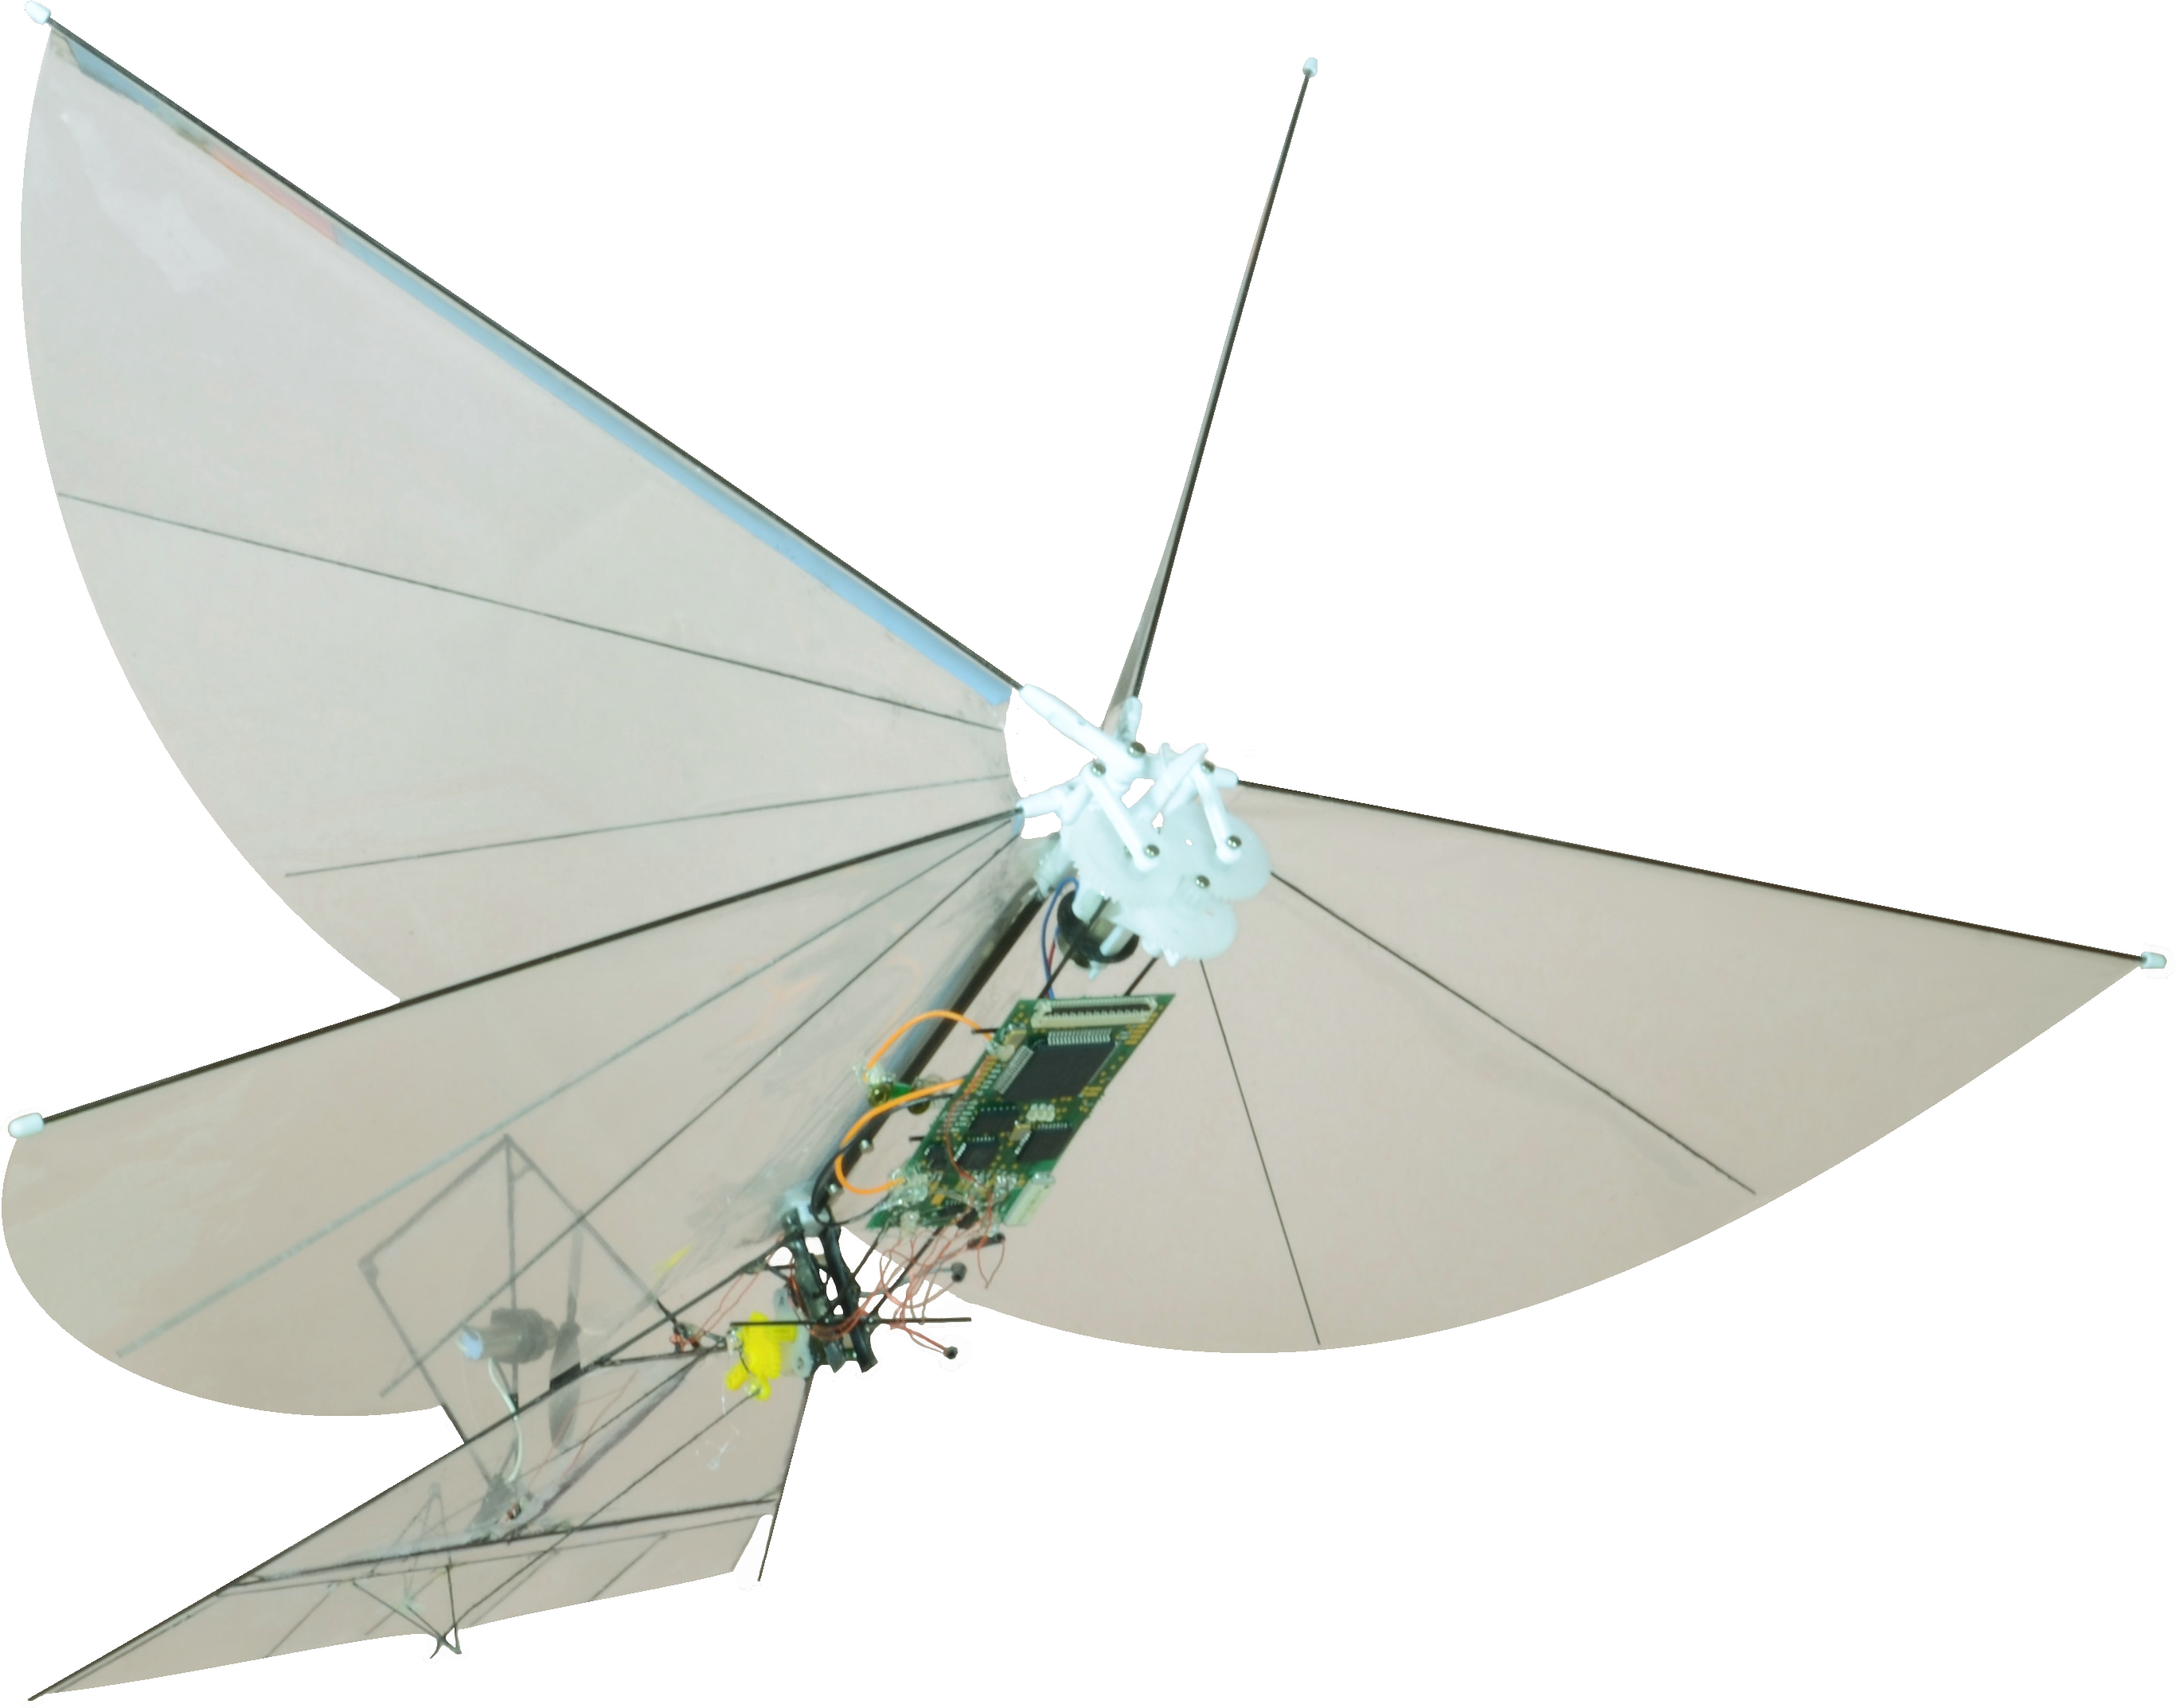
\includegraphics[width=\linewidth]{figures/h2bird.png}
\caption{H$^2$Bird ornithopter MAV}
\label{fig:h2bird}
\end{figure}
Power, size, and weight constraints on micro air vehicles (MAV) 
significantly limit their sensing and computational capabilities. They can 
execute only the most rudimentary control and state estimation algorithms in 
real-time.  The constraints on flapping-wing MAVs are even more restrictive. 
Though they demonstrate safety and noise profiles superior to those of 
rotorcraft MAVs, this comes at the expense of reduced payload.

The non-linear dynamics of flapping-wing flight compound 
these constraints~\cite{humbert:dipteran2}\cite{cheng:tandrdamping}. Much 
past research on flapping-wing MAVs focuses on overcoming the difficulties 
of controlling and modeling flapping-wing vehicles in the face of this
non-linearity\cite{floreano:flying}. Common approaches to simplify these 
dynamic models include averaging over the wing-beat 
period~\cite{Schenato:flightcontrol}\cite{cheng:tandrdamping}, and using 
linear, low-dimensional models to predict flight 
behavior~\cite{Shigeoka:ornithopter}. These advances lead to the development 
of high-performance platforms such as the sub-15 gram DelFly, described by 
deCroon et al.~\cite{delfly:design}. 

Many control laws previous researchers developed from dynamic models of 
flapping-wing flight, such as periodic forcing and other control methods 
described by~\cite{doman:dynamics}\cite{khan:longitudinal_control}\cite{leonard:averaging}, 
require powerful on-board computing. In this work, we develop a simpler, 
less computationally-intensive method of control for negotiating narrow 
passages, by exploiting cooperation between specialized robotic agents.

In contrast to flight control, there is considerably less previous work on 
guidance and navigation of flapping-wing MAVs. Baek demonstrated altitude 
control with an external camera~\cite{baek:altitude}. de Croon et al. 
demonstrated obstacle avoidance with an onboard camera and offboard 
processing~\cite{delfly:avoid}. Baek et al. provide one of the few examples 
of completely autonomous target seeking for vehicles at the sub-20 gram 
scale~\cite{baek:tracking}.

There also exists a body of work on the guidance and control of fixed- and 
rotary-wing MAV platforms, but many of these methods make extensive use of 
GPS or motion capture systems~\cite{kingston:timeattitude}\cite{kanade:3dvision}. 
Indoors, using GPS to estimate the pose of an MAV is impossible, and motion 
capture requires extensive and stationary modification of the environment. 
The power and payload limits on flapping-wing MAVs make complex on-board 
sensing difficult, so multiagent cooperative control schemes are apt 
solutions.

The literature on cooperative control of MAVs is similarly limited to larger
vehicles and purely analytical explorations. Nebot, Hyams, and Jung all 
demonstrated cooperative visual servoing for heterogeneous UGVs~\cite{Nebot2003Agents}\cite{Hyams1999Cooperative}\cite{Jung1998Range}. 
Luo and Mehta analyze  UAV-UGV cooperation from a modeling perspective~\cite{Luo2011Air}\cite{Mehta2006Adaptive}. 
Rudol demonstrated a cooperative visual servoing system similar with 
UGVs and MAVs~\cite{Rudol2008Micro}, but the vehicles used were orders of 
magnitude larger than the millirobotic systems we target, and so were able 
to take advantage of high-performance processors and specialized cameras.

The small size of millirobotic air and ground vehicles necessitates 
specialization, but it also pays dividends agility. A group of specialized 
heterogeneous millirobots can navigate more challenging terrains and 
interact with their environments in ways that larger, monolithic vehicles 
cannot. Despite this advantage, in order to collectively equal the sensing and 
computational capabilities of larger robots, they will also have to interact 
so that multiple robots can benefit from the specialized capabilities of 
cooperating vehicles. Millirobotic systems will benefit from cooperation 
even more than their larger counterparts. 

%%%%%%%%%%%%%%%%%%%%%%%%%%%%%%%%%%%%%%%%%%%%%%%%%%%%%%%%%%%%%%%%%%%%%%%%%%%%%%
\section{Robotic and Vision Platforms}
%----------------------------------------------------------------------------%
\subsection{H$^2$Bird Ornithoper}
% humphrey
To explore these cooperative control concepts, we designed a new 
flapping-wing MAV, known as the H$^2$Bird (Fig.~\ref{fig:h2bird}). Built 
around the Silverlit i-Bird RC flyer power train and clap-fling wings\footnote{\raggedright Silverlit Toys Manufactory Ltd.: i-Bird RC Flyer
\href{http://www.silverlit-flyingclub.com/wingsmaster/}
     {http://www.silverlit-flyingclub.com/wingsmaster/}}, 
the H$^2$Bird has a wingspan of 26.5 cm and a flight weight of 13 grams. A 
tail propeller and servo-controlled tail elevator provide control in the yaw 
and pitch axes (Fig.~\ref{fig:h2Bird_axes}). The on-board ImageProc 2.4\footnote{ImageProc 2.4: \\
\href{https://github.com/biomimetics/imageproc\_pcb}
     {https://github.com/biomimetics/imageproc\_pcb}} 
controller includes of a 40 MIPS microprocessor, 6 DOF IMU, 
IEEE 802.15.4 radio, VGA camera, and motor drivers, all powered by a 90 mAh 
lithium polymer battery. In routine flight, the H$^2$Bird averages 1.2 m/s 
ground speed, and operates for approximately 10 minutes.

%----------------------------------------------------------------------------%
\subsection{Ground Station Computer Vision Platform}
% ryan
Cooperative behavior is a promising strategy for autonomous navigation in 
unexplored and unstructured environments. However, to operate in these 
environments, a cooperative system must be fully mobile, not tied to a 
static ground station or motion capture laboratory. To demonstrate the 
feasibility of this approach, we designed our ground station to conform to 
the power and weight constraints of highly mobile millirobotic ground 
vehicles, such as OctoRoACH, which can traverse rough terrains with speed and 
agility~\cite{Pullin2012Dynamic}. 

Rather than power-intensive PC processors, we used the ARM-based BeagleBoard 
single-board computer as a reference computation platform. The BeagleBoard 
consumes approximately one watt while running our computer vision and 
control algorithms. It uses the same processor as popular sub-10 gram 
processor modules--such as the Gumstix Overo and LogicPD Torpedo--which are 
light enough for deployment on millirobotic ground vehicles. We pair the 
BeagleBoard with an off-the-shelf consumer USB web camera, for similar image 
quality and resolution to the miniature camera modules available at 
millirobot scale. The BeagleBoard communicates with the H$^2$Bird with a 
USB radio module which implements the IEEE 802.15.4 wireless standard.
%TODO footnotes: Gumstix, LogidPD

Our ground station software is based on the Ubuntu Linux\footnote{\raggedright Ubuntu: 
Canonical Ltd., \href{http://www.ubuntu.com/}{http://www.ubuntu.com/}} distribution
modified with a custom version of the Linux kernel. 
We use the Python\footnote{\raggedright Python: Python Software Federation, \href{http://www.python.org/}
{http://www.python.org/}} programming language for control, robot 
communication, and telemetry, and the OpenCV\footnote{\raggedright OpenCV: Willow Garage, 
\href{http://opencv.willowgarage.com/wiki/}{http://opencv.willowgarage.com/wiki/}} 
computer vision libraries for image capture and processing.
%%%%%%%%%%%%%%%%%%%%%%%%%%%%%%%%%%%%%%%%%%%%%%%%%%%%%%%%%%%%%%%%%%%%%%%%%%%%%%
\section{System Concept and Algorithms}
%TODO ryan

\begin{figure}[tb]
\centering
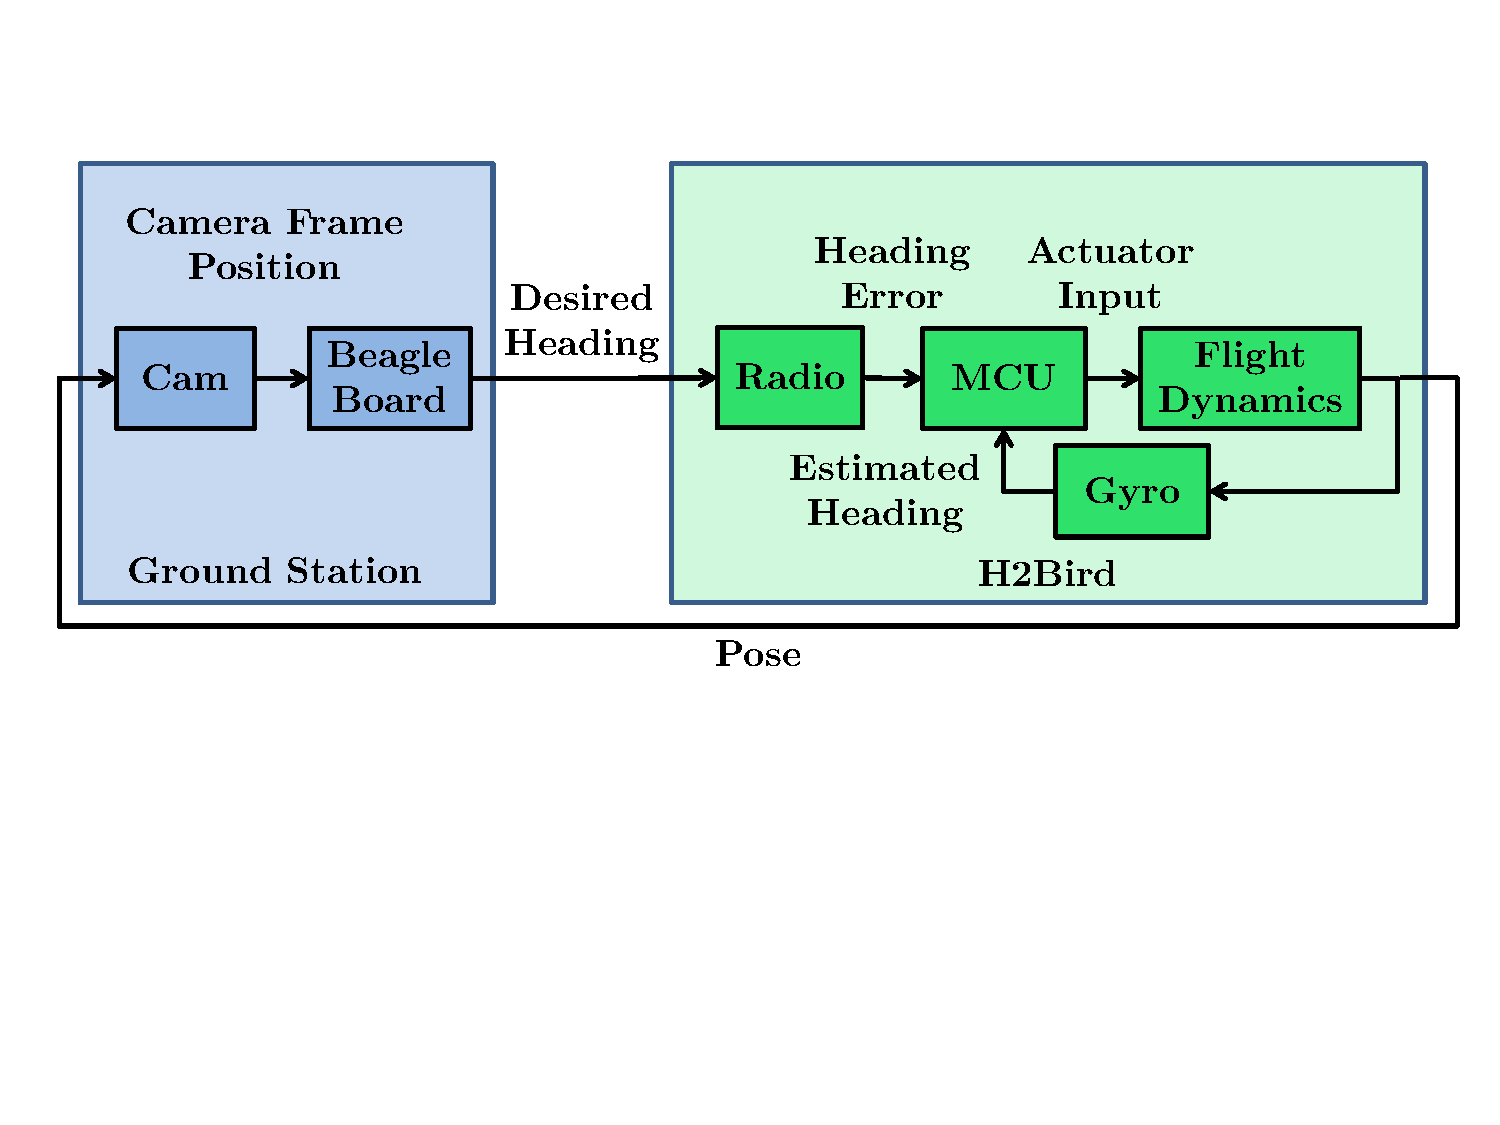
\includegraphics[width=\linewidth]{figures/process_flow.pdf}
\caption{Overview of the cooperative control system.}
\label{fig:process_flow}
\end{figure}
%TODO h2bird label in diagram should have superscript

%----------------------------------------------------------------------------%
\subsection{Ornithoper Attitude Control}

\begin{figure}[!tb]
\centering
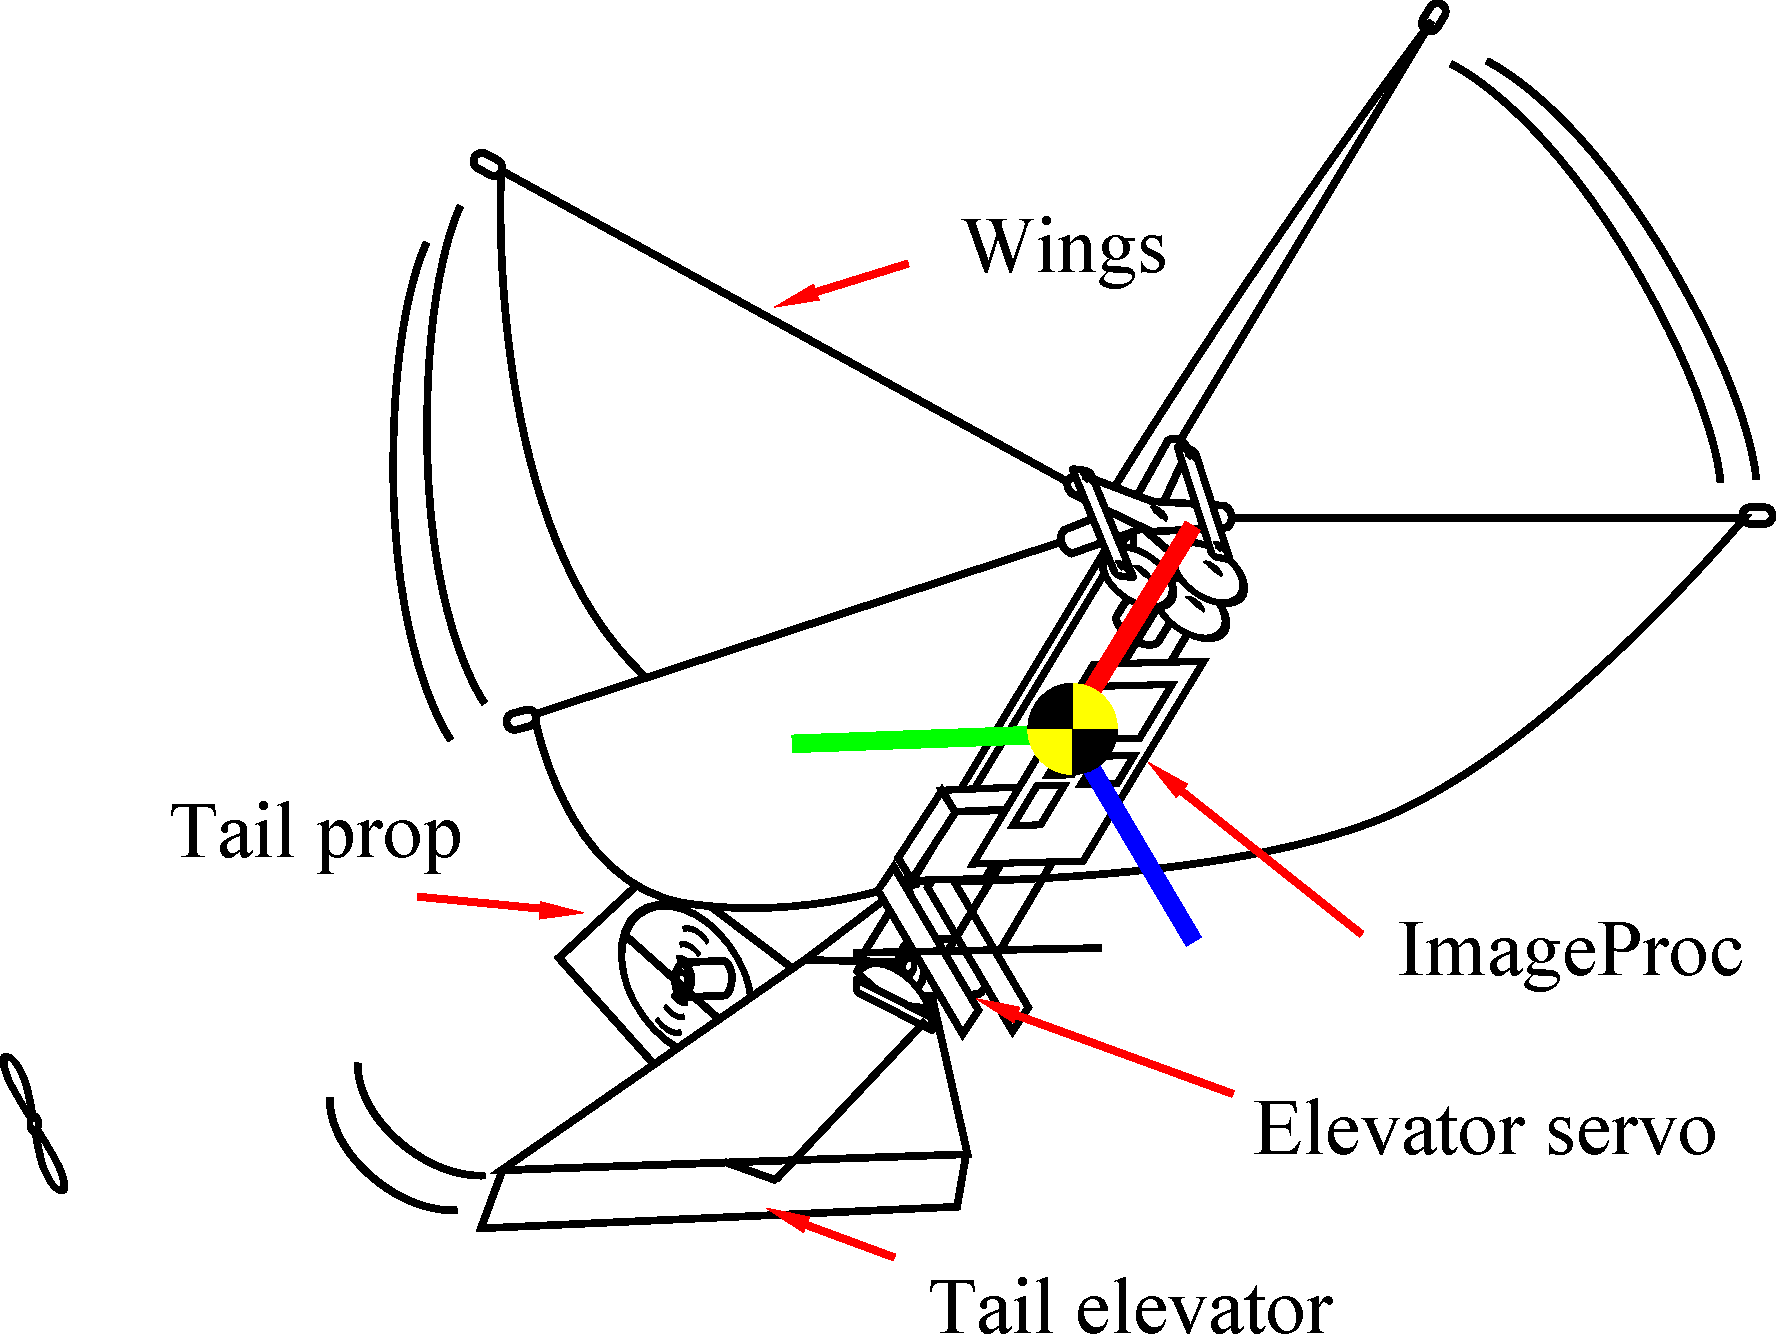
\includegraphics[height=150pt]{figures/h2bird_axes.pdf}
\caption{H$^2$Bird ornithopter with attitude control axes and labeled 
control surfaces.}
\label{fig:h2Bird_axes}
\end{figure}
%TODO label h2bird drawing

We implement attitude estimation and control of the H$^2$Bird on-board to 
achieve high sample-rate attitude control. We estimate the vehicle pose by
integrating the IMU, and use a proportional-integral-derivative (PID) 
controller to feed these estimates back to the attitude control flight 
surfaces (Figs.~\ref{fig:process_flow} and~\ref{fig:block_diagram}).

The high pitch angles at which flapping-wing MAVs regularly operate 
distinguish them from other MAVs. Baek demonstrated control on a similar 
vehicle using PID and an Euler angle parameterization of orientation~\cite{baek:tracking}. 
However, Euler angle parameterizations of vehicle orientation suffer from 
singularities around high pitch angles. So we instead represent the vehicle 
orientation with quaternions. The quaternion representation allows us to 
represent relative body and world coordinate angular displacements compactly 
with quaternion multiplication.

Our implementation of quaternion-based control is similar to 
Knoebe's~\cite{knoebe:quatcontrol}:
Given a reference pose represented in quaternion form $q_r$, we define the 
error as the rotation $q_e$ required to reach the reference pose from the 
estimated pose $q$ (Eq.~\ref{eq:quat_error}). 
\begin{align}
\label{eq:quat_error}
q_e &= q^{\prime}\cdot q_r \\
		&= q_{e,w} + q_{e,x}\hat{i} + q_{e,y}\hat{j} + q_{e,z}\hat{k} \notag 
\end{align}
We then convert this error quaternion to an angle axis representation and 
use it as input to the PID controller (Eqs.~\ref{eq:quat_linearize} and~\ref{eq:quat_angle}).
We perform these calculations on-board, with trigonometric lookup tables for 
real-time performance.
\begin{align}
\label{eq:quat_linearize}
Q_e &= \alpha\cdot q_e/\sin(\alpha /2) \\
		&= \alpha_{x}\hat{i} + \alpha_{y}\hat{j} + \alpha_{z}\hat{k} \notag
\end{align}
\begin{equation}
\label{eq:quat_angle}
\alpha = 2\arccos(q_{e,w})
\end{equation}

%----------------------------------------------------------------------------%
\subsection{Ground Station Pose Estimation}
The ground station performs simple two-dimensional pose estimation on 
H$^2$Bird using a particle filter-based motion tracking algorithm. This pose 
estimate is the feedback input to the cooperative visual servoing feedback 
loop, which is represented as the outermost feedback paths on the block 
diagrams in Figs.~\ref{fig:process_flow} and~\ref{fig:block_diagram}. We 
limit our pose estimation approach to monocular two-dimensional object 
tracking in pixel space. This allows us to perform real-time video tracking 
using the modest computational resources available on the ground station, 
and similarly, millirobotic ground vehicles.

Our pose estimation algorithm tracks H$^2$Bird's motion in the frame using a 
particle filter~\cite{thrun2005probabilistic}. We initialize the particles 
uniformly across the frame before tracking begins. To improve numerical 
stability, we normalize the weights of all particles on each iteration, and 
only resample the particle population when the mean particle weight falls 
below a pre-determined threshold. 
%............................................................................%
\subsubsection{Motion Model}
Our motion model (Eq.~\ref{eq:motion_model}) is a simple Gaussian transition 
centered around each particle's current position, augmented with an 
$\epsilon$-random uniform sampling strategy. In Eq.~\ref{eq:motion_model}, 
$x^{[i]}_t$ is the position of the $i^\text{th}$ particle in pixel space at 
time $t$, $\Sigma$ is a chosen covariance matrix, and $b$ is a vector of the 
bounds of the pixel space.
\begin{equation}
\label{eq:motion_model}
x^{[i]}_t \sim \begin{cases}
\mathcal{N}(x^{[i]}_{t-1}, \Sigma), &\text{with probability } 1-\epsilon \\
\mathcal{U}(0,b),& \text{with probability } \epsilon \\
\end{cases}\\
\end{equation}
In the experiments we present in this work, we used a diagonal covariance matrix 
with a variance of 256, and an $\epsilon$ of 0.3. We find the Gaussian 
transition model is sufficient for tracking motion in which frame-to-frame 
position changes are relatively small. The $\epsilon$-random uniform 
transitions increase tracking robustness, by forcing the filter to always 
sample broadly across of the pixel space. This helps prevent overconfidence 
and collapse, and decreases reacquisition delay. 

%............................................................................%
\subsubsection{Emission Model}
Our emission model (Eq.~\ref{eq:emission_model}) implements a sampling
approach to motion tracking via na\"{i}ve background subtraction, e.g. frame 
differencing~\cite{Ahad2011Computer}. On each iteration, the system provides the emission 
model with $f_0$, the frame representing the background, and $f_t$, the most 
recent frame captured. The model assigns a weight $w^{[i]}_t$ to each 
particle $x^{[i]}_t$, proportional to the color distance in RGB space 
between the pixels of $f_0$ and $f_t$ at the location $x^{[i]}_t$.
\begin{equation}
\label{eq:emission_model}
w^{[i]}_t = 1 + \norm{f_0(x^{[i]}_t)-f_t(x^{[i]}_t)}^2
\end{equation} 
Hence, particles are more likely to be resampled in regions of 
the image which are dissimilar in color from the background.

During the experiments presented in this work, we assumed that neither the 
bird, nor any other moving object, were visible in the frame on system 
start. We saved the first frame captured by the system, and provided it as 
the background frame $f_0$ for every iteration of the particle filter. This 
choice of $f_0$ resulted in a sampling approach to na\"{i}ve background 
subtraction. 

Na\"{i}ve background subtraction is brittle to changes in a scene over 
time~\cite{Ahad2011Computer}. However, we find it very efficient, and sufficiently 
reliable for the short time spans--less than five seconds--necessary for 
H$^2$Bird to successfully negotiate narrow openings. Calculating $f_0$ 
using a more sophisticated background extraction would retrain the 
underlying motion tracking features of the filter, while providing the 
algorithm with a more robust way of differentiating subject motion from the 
background.

%----------------------------------------------------------------------------%
\subsection{Cooperative Visual Servoing}
\label{sec:visual_servoing_concept}
The ground station guides the H$^2$Bird by commanding changes to its 
reference attitude, which is in turn governed by its on-board attitude 
controllers (Figs.\ref{fig:process_flow} and~\ref{fig:block_diagram}). Using 
the estimate of 2D vehicle pose from the pose estimation algorithm, the 
ground station calculates an altitude error and horizontal error. The ground 
station then commands a reference attitude to the H$^2$Bird over radio, 
according to a PID control law. We apply a fixed-lag window the PID 
controller integral term to prevent wind-up while we launch the ornithopter. 
We tuned the proportional and derivative terms of this outer controller to 
dampen the overshoot and drift caused by the cooperative system latency.
\begin{figure}[tb]
\centering
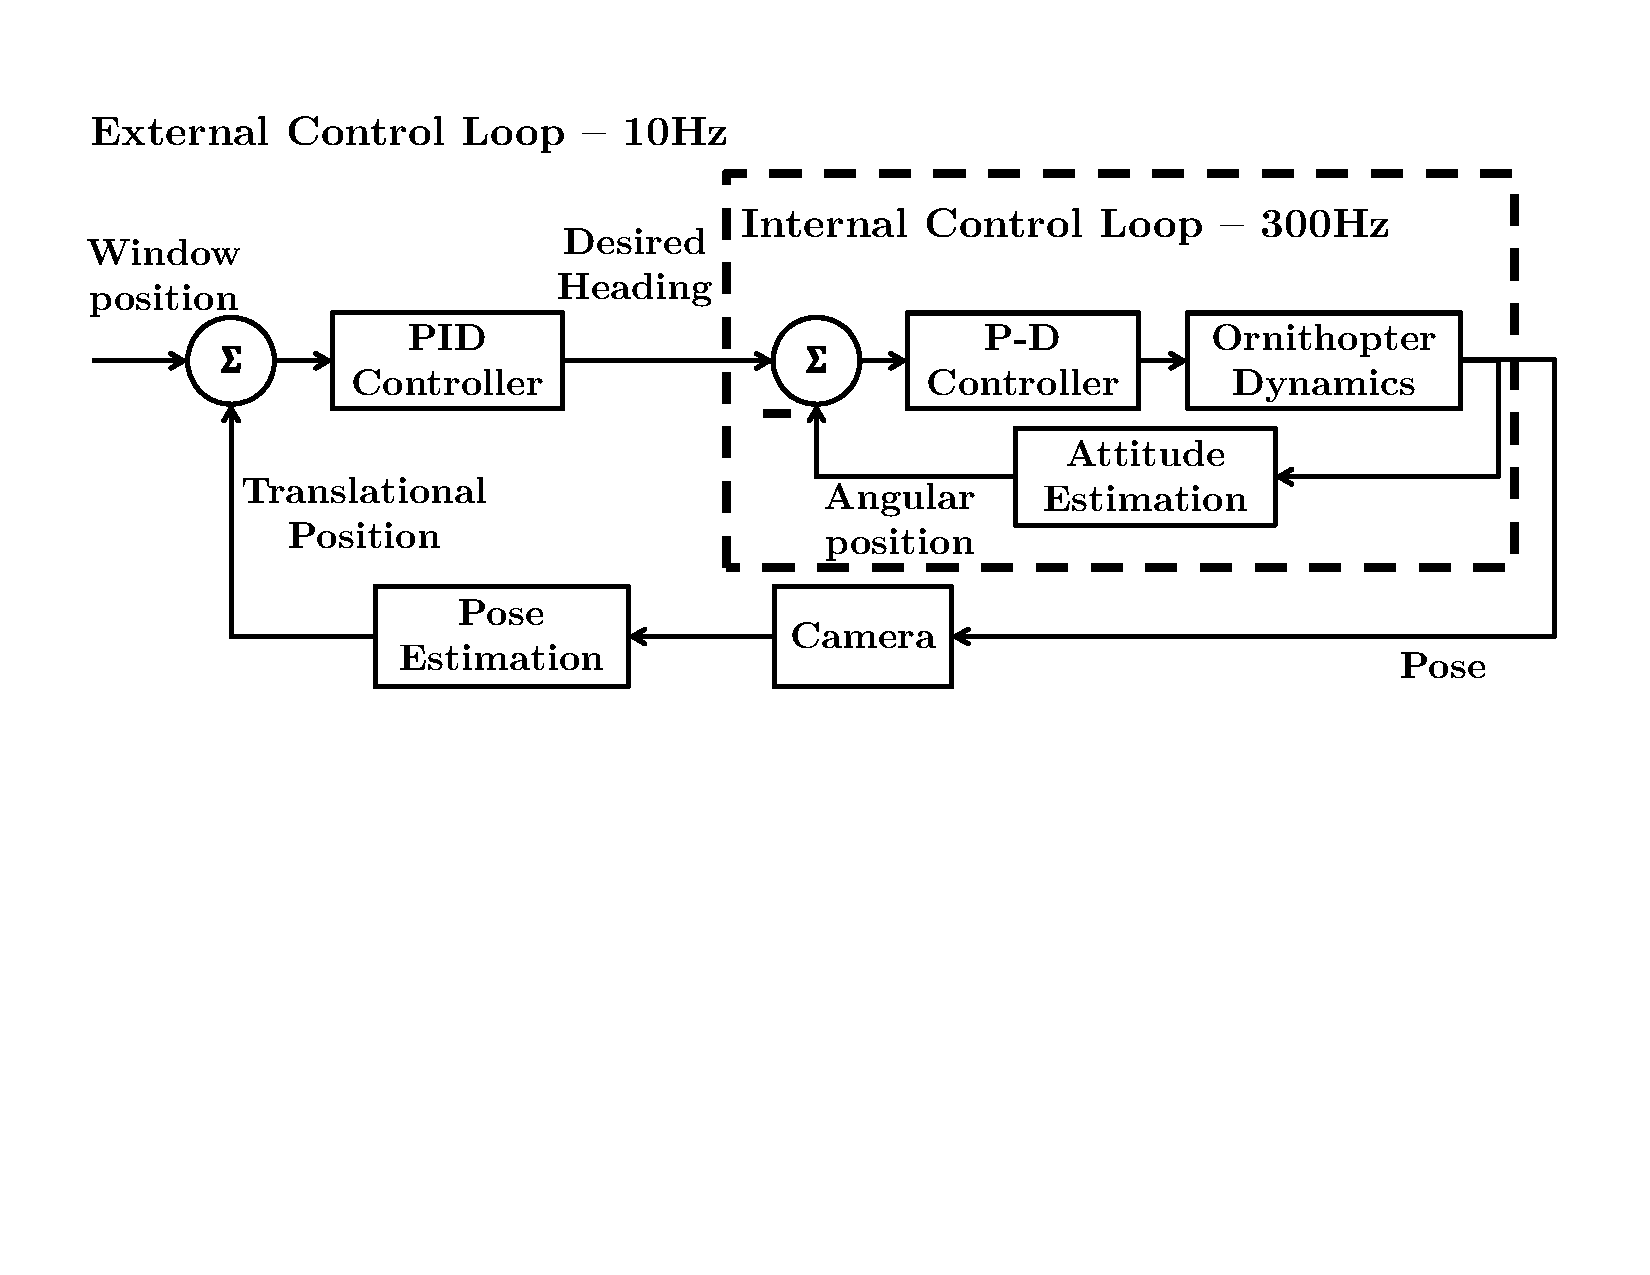
\includegraphics[width=\linewidth]{figures/block_diagrams.pdf}
\caption{Overall block diagram of the cooperative control system.}
\label{fig:block_diagram}
\end{figure}

%%%%%%%%%%%%%%%%%%%%%%%%%%%%%%%%%%%%%%%%%%%%%%%%%%%%%%%%%%%%%%%%%%%%%%%%%%%%%%
\section{System Model}
\label{sec:system_model}

%----------------------------------------------------------------------------%
\subsection{Ornithopter Attitude Control}
\label{sec:model_attitude}

We divide our model of the vehicle pose into two independent models for 
simplicity: one for yaw motion, and one for translational motion.

We approximate the yaw dynamics of the ornithopter with a one-dimensional 
model to limit complexity, and because it matches our physical 
implementation. Likewise, we choose the reference heading angle as input to 
the model, and model the dynamics of vehicle and on-board PID controller as 
one system, whose output is the physical heading angle. We show the 
resulting model form in Equation~\ref{eq:plain_model}.
\begin{equation}
\label{eq:plain_model}
H(s) = \frac{K}{1 + Rs}
\end{equation}
To model the translational position of the ornithopter, we use a form of 
Dubin's car model (Eq.~\ref{eq:dubin_car})~\cite{lavalle:planning}, where 
$\phi_{max}$ is the maximum steering angle and $u_{s}$ is the forward speed. 
\begin{equation}
\label{eq:dubin_car}
\begin{aligned}
& \dot{x} = u_{s}sin(\theta)\\
& \dot{y} = u_{s}cos(\theta)\\
& \dot{\theta} = u\\
& u \in U=[-\tan{\phi_{max}},\tan{\phi_{max}}]
\end{aligned}
\end{equation}
We modify this model to treat the angular position $\theta$ as an input 
rather than a state. The overall motion of the system can be modeled as shown 
in Equation~\ref{eq:dubin_car}, where $\theta$ is the time-domain output of 
Equation~\ref{eq:plain_model} with the reference heading angle as input.

%----------------------------------------------------------------------------%
\subsection{Ground Station Pose Estimation}

Our model of the ground station comprises models of both the camera and the
pose estimation computation. The camera model contains both a latency, which 
is in series with the path between the ``Camera'' and 
``Ornithopter Dynamics'' blocks in Figure~\ref{fig:block_diagram}, and a 
model of the camera's viewing angle constraints.
 
We model the viewing angle of the camera as a pixel map from one edge of a 
63$^{\circ}$ viewing triangle to the other. The camera has an image width of 
640 pixels. We calculate the desired heading angle in degrees, for a given 
distance from the camera, according to Equation~\ref{eq:desired_heading}.
\begin{equation} 
\label{eq:desired_heading} 
\text{Desired heading} = \frac{640\,\text{px}}{2d\tan{\frac{63^{\circ}}{2}}}{\times\frac{63^{\circ}}{640\,\text{px}}\times x}
\end{equation}
where $d$ is the distance between the ornithopter and the camera, and $x$ is 
the horizontal position of the robot relative to the center of the window in 
meters. This relation reflects the fact that the pose estimation algorithm 
does not determine the depth of the robot, which can be problematic for 
control algorithms. For example, if the ornithopter remains at a constant 
horizontal distance from the window, but moves closer and closer to the 
camera, the ground station's directed heading steadily increases, even 
though the robot has not actually moved farther from the window. These 
problems are most severe in areas close to the camera.

We model the pose estimation computation delay, which include the latency of 
updating the particle filter, calculating a new reference attitude, and 
sending the reference attitude command the ornithopter via radio.

%%%%%%%%%%%%%%%%%%%%%%%%%%%%%%%%%%%%%%%%%%%%%%%%%%%%%%%%%%%%%%%%%%%%%%%%%%%%%%
\section{Experiments}

%----------------------------------------------------------------------------%
\subsection{System Identification}

%............................................................................%
\subsubsection{Ornithoper Attitude Control}
We determined the turning speed and turning radius of the H$^2$Bird 
experimentally, by measuring the response of the system to a step input of a 
clockwise 90$^{\circ}$ turn. We measured the response of the system by 
recording the attitude estimates calculated by the ornithopter using its 
on-board gyroscope. We then used MATLAB\footnote{The MathWorks, Inc. Matlab:
\href{http://www.mathworks.com/products/matlab/}
     {http://www.mathworks.com/products/matlab/}} 
to fit a simple low-order model to the step response, as discussed in 
Sec.~\ref{sec:model_attitude}.

%............................................................................%
\subsubsection{Ground Station Pose Estimation}
To measure the capture latency of the camera, we wrote a simple test 
application which draws a large colored rectangle on the ground station's 
screen, then uses the camera to detect that changes in that rectangle's 
color. By noting the value of the system timer just before it changes the 
rectangle, and just after the camera detects that change, the application 
arrives at an estimate of the video capture pipeline latency. We averaged 
these result over several hundred rapidly-executed trials to determine the 
capture latency we used to model the system.

To compute the particle filter and controller latency, we again used system 
timers to determine the average time between the start and end of computation.

%----------------------------------------------------------------------------%
\subsection{Model Verification}
\label{sec:experiments_verification}

We tested our cooperative visual servoing system with a simple target seeking
experiment: the H$^2$Bird must fly through a specified obstacle, in this 
case, a wooden frame we used to simulate a window.

\begin{figure}[tb]
\centering
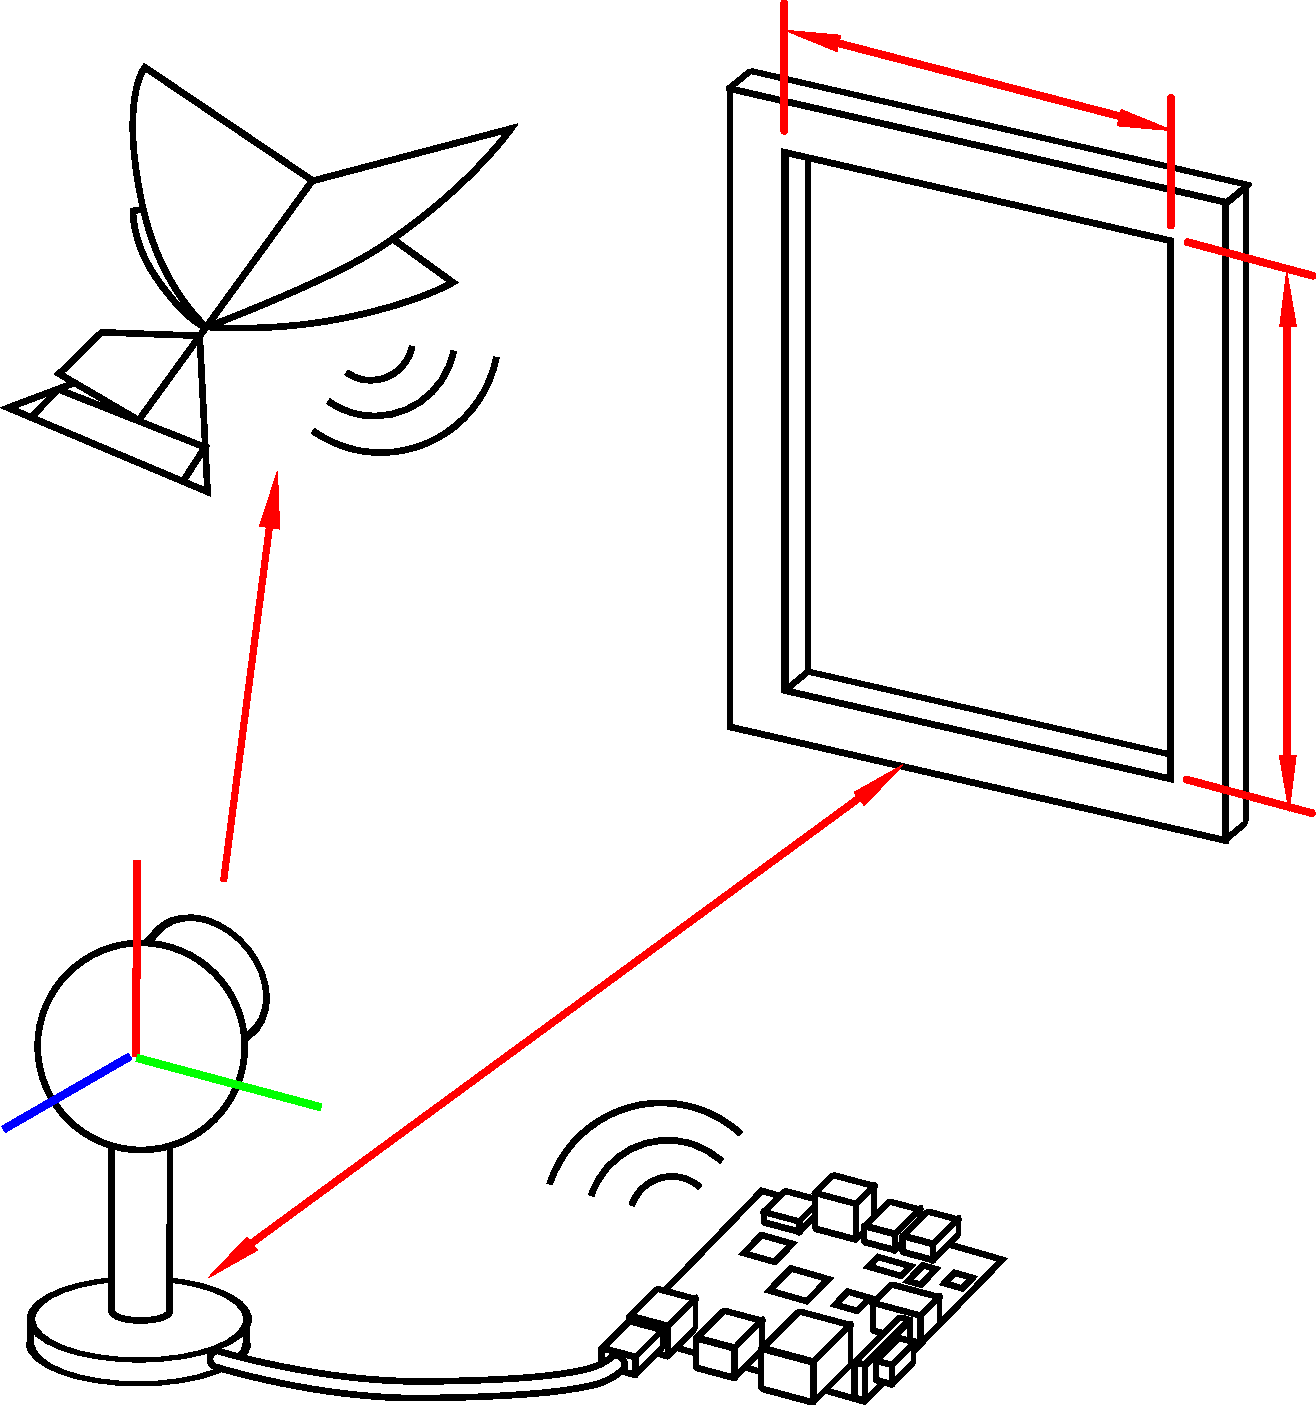
\includegraphics[width=\linewidth]{figures/experiment_cartoon.pdf}
\caption{Conceptual sketch of experimental setup.}
\label{fig:experiment_cartoon}
\end{figure}

As the H$^2$Bird cannot detect the target on its own, we used cooperative 
control with the ground station, which to provided remote guidance to 
H$^2$Bird to allow it to navigate to the window. We used a motion capture 
system to record ground truth data. We present a sketch of this experimental 
setup in Figure~\ref{fig:experiment_cartoon}.

\begin{figure}[tb]
\centering
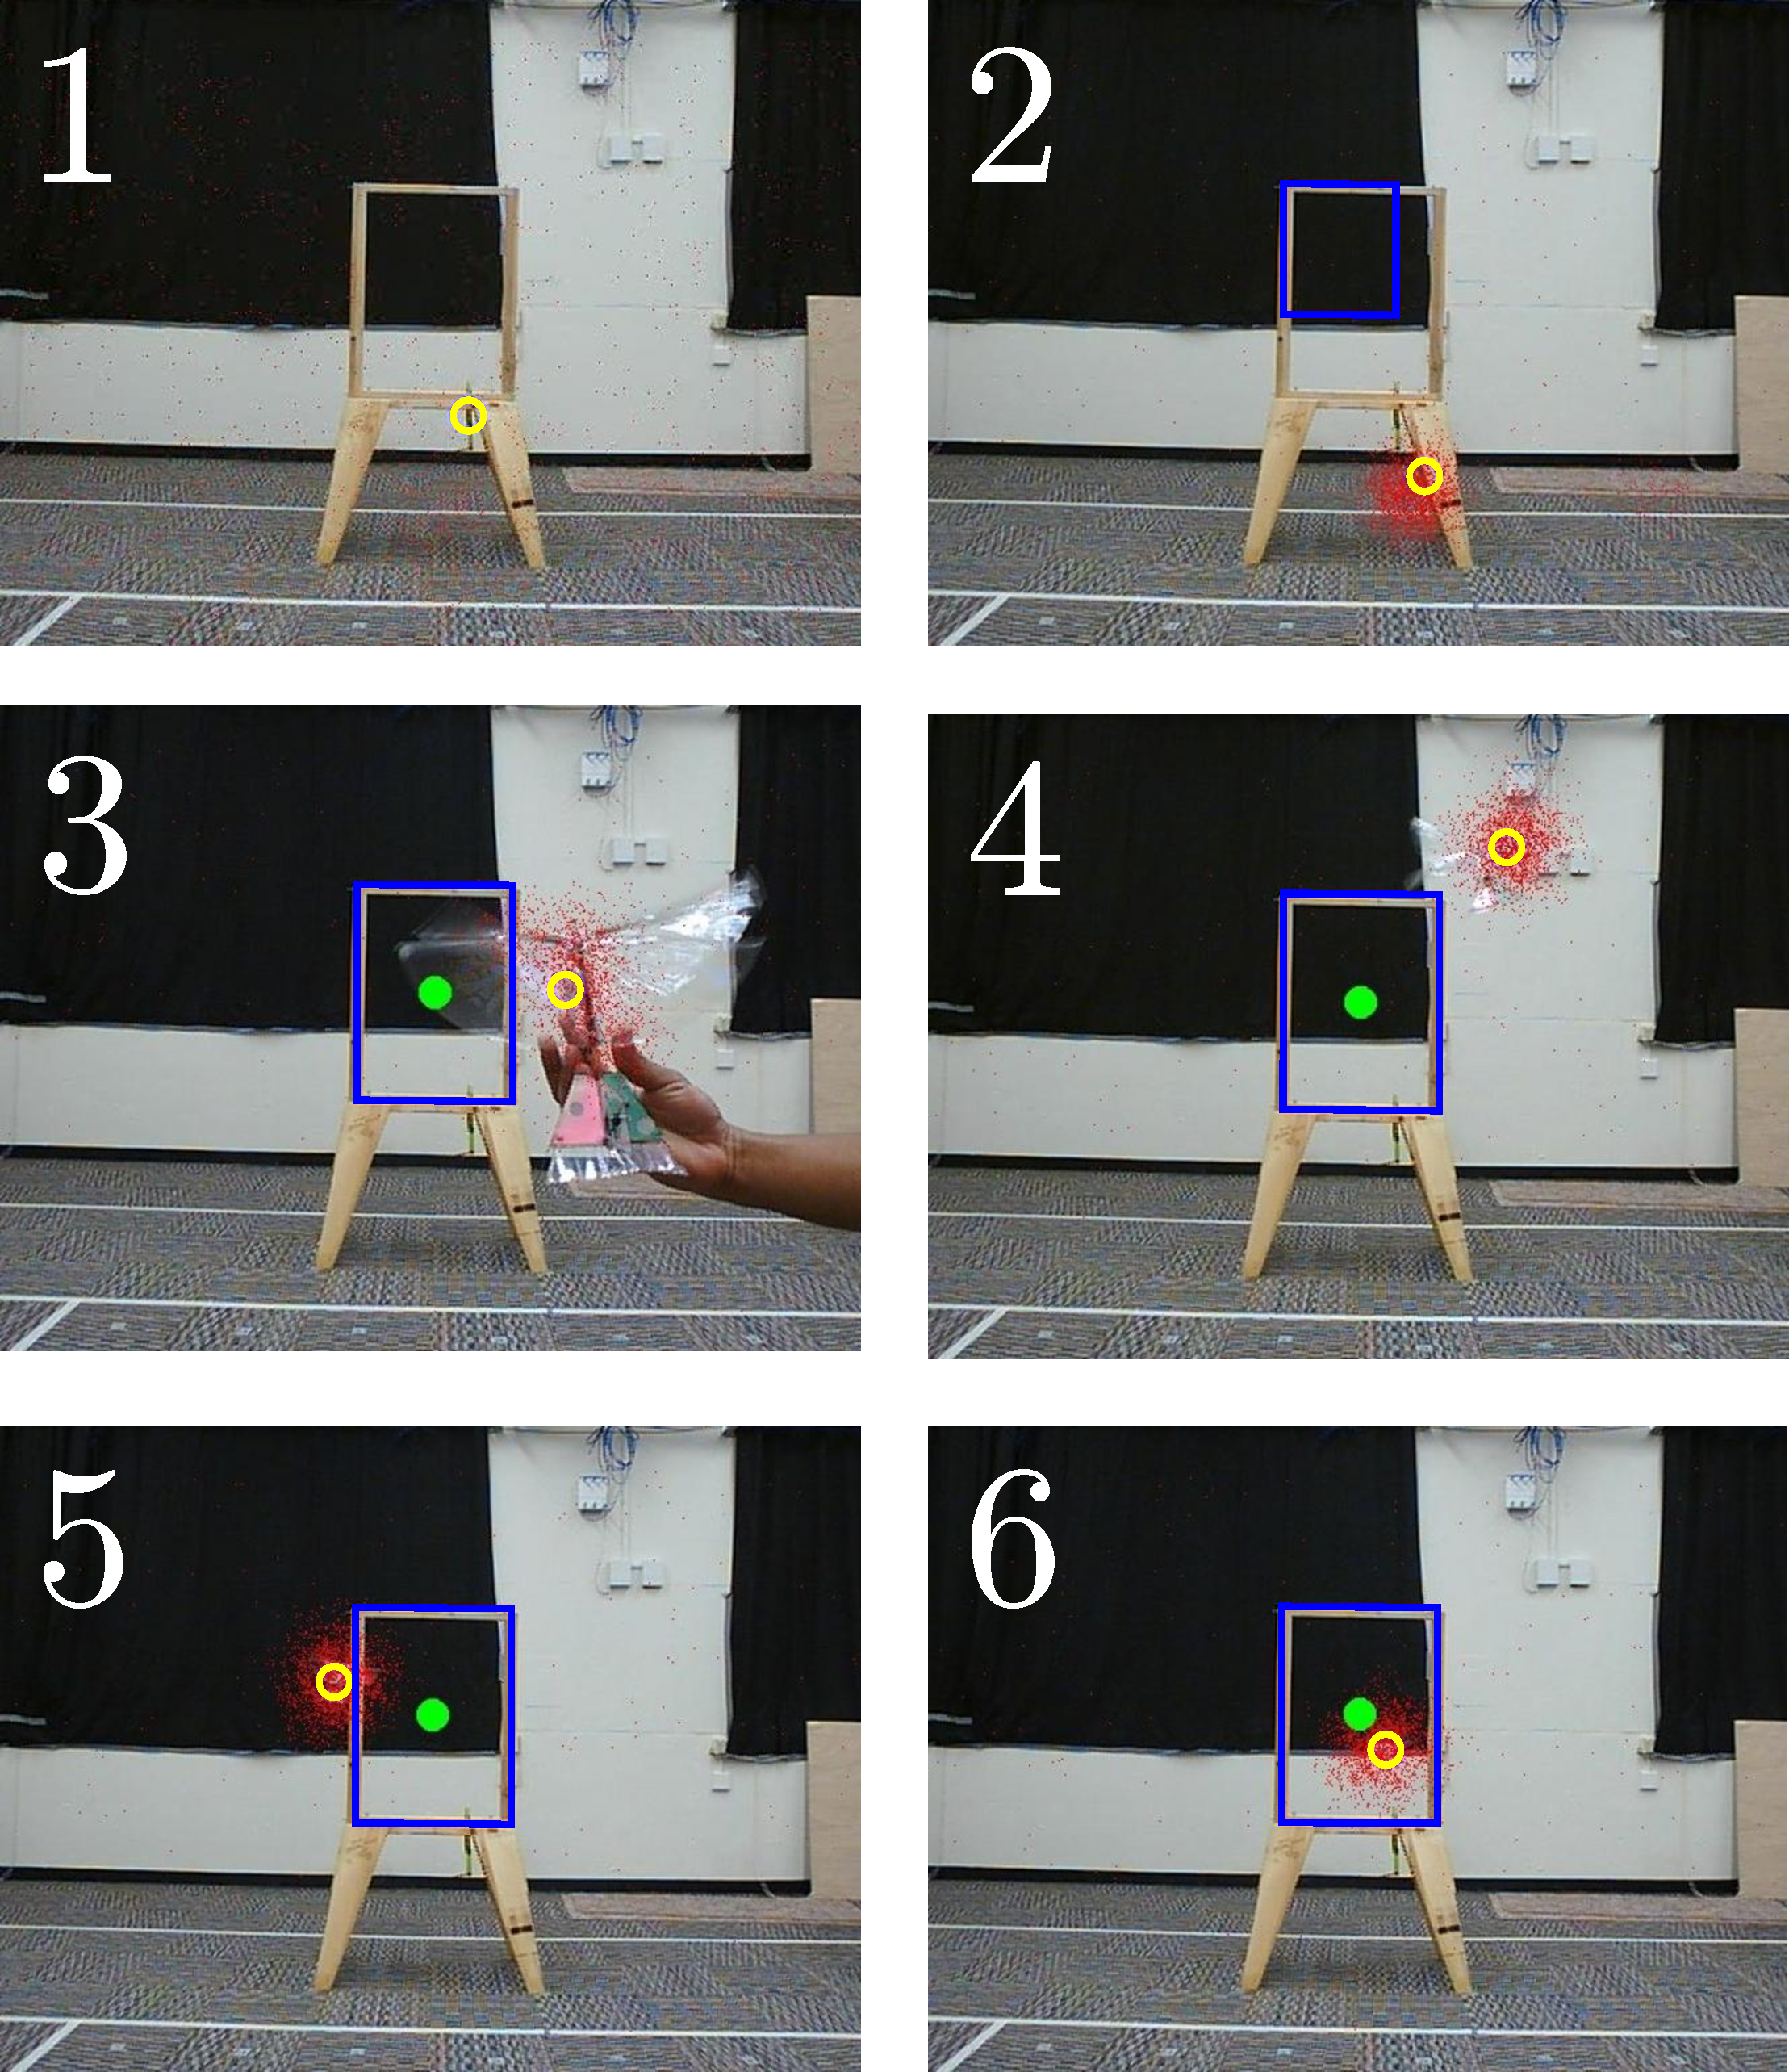
\includegraphics[width=\linewidth]{figures/pf_screencap.pdf}
\caption{Frame sequence from video feed used for tracking. Particles 
are shown in \textcolor{red}{red}, the current state estimate as a 
\textcolor{yellow}{yellow} circle, the window bounding box in
\textcolor{blue}{blue}, and the target location as a \textcolor{green}{green} 
circle. 1.~Particles initialized uniformly across the frame; 2.~Human operator 
dragging bounding box across the window; 3.~H$^2$Bird enters the frame. 
Particles converge on its location; 4.~Release H$^2$Bird, which 
begins cooperative autonomous flight toward the target; 5.~Visual servoing 
controller overshoots the window on the left, and commands a right-turn 
maneuver to recover; 6.~H$^2$Bird successfully navigates through the window.}
\label{fig:pf_screencap}
\end{figure}

Each trial included the following steps (see Fig.~\ref{fig:pf_screencap}):
\begin{enumerate}
\item We identify the window to the ground station by dragging a bounding 
box over it using the mouse. 
\item We release H$^2$Bird by hand, in view of the camera at the desired 
starting grid point.
\item The H$^2$Bird attempts to fly through the window with, with remote 
guidance from the ground station.
\end{enumerate}

After every 5 trials, we replaced the ornithopter's battery with a fully 
charged one.

In total, we collected 80 trials over a variety of starting positions. Our 
goal for these experiments was to verify the model described in 
Section~\ref{sec:system_model}, so we conducted 60 of the 80 trials in a 
grid along the edges of the camera view plane, and in 5 cm meter increments 
from the window, in an effort to determine the success rate on the edges of 
the testing space. We conducted 20 additional trials directly in front of 
the camera, to determine the success rate near the center of viewing plane. 

%%%%%%%%%%%%%%%%%%%%%%%%%%%%%%%%%%%%%%%%%%%%%%%%%%%%%%%%%%%%%%%%%%%%%%%%%%%%%%

%%%%%%%%%%%%%%%%%%%%%%%%%%%%%%%%%%%%%%%%%%%%%%%%%%%%%%%%%%%%%%%%%%%%%%%%%%%%%%
\section{Results and Performance}
\label{sec:performance}
%TODO cameron
To bound the performance of the cooperative control system, we determine 
the feasible set of initial conditions that result in successful narrow 
passage traversal, using both analytical and empirical methods. We then 
conduct experiments to validate this model.

%----------------------------------------------------------------------------%
\subsection{System Identification}

%............................................................................%
\subsubsection{Ornithoper Attitude Control}
\label{sec:flight_control}
%TODO cameron
\begin{figure}[tb]
\centering
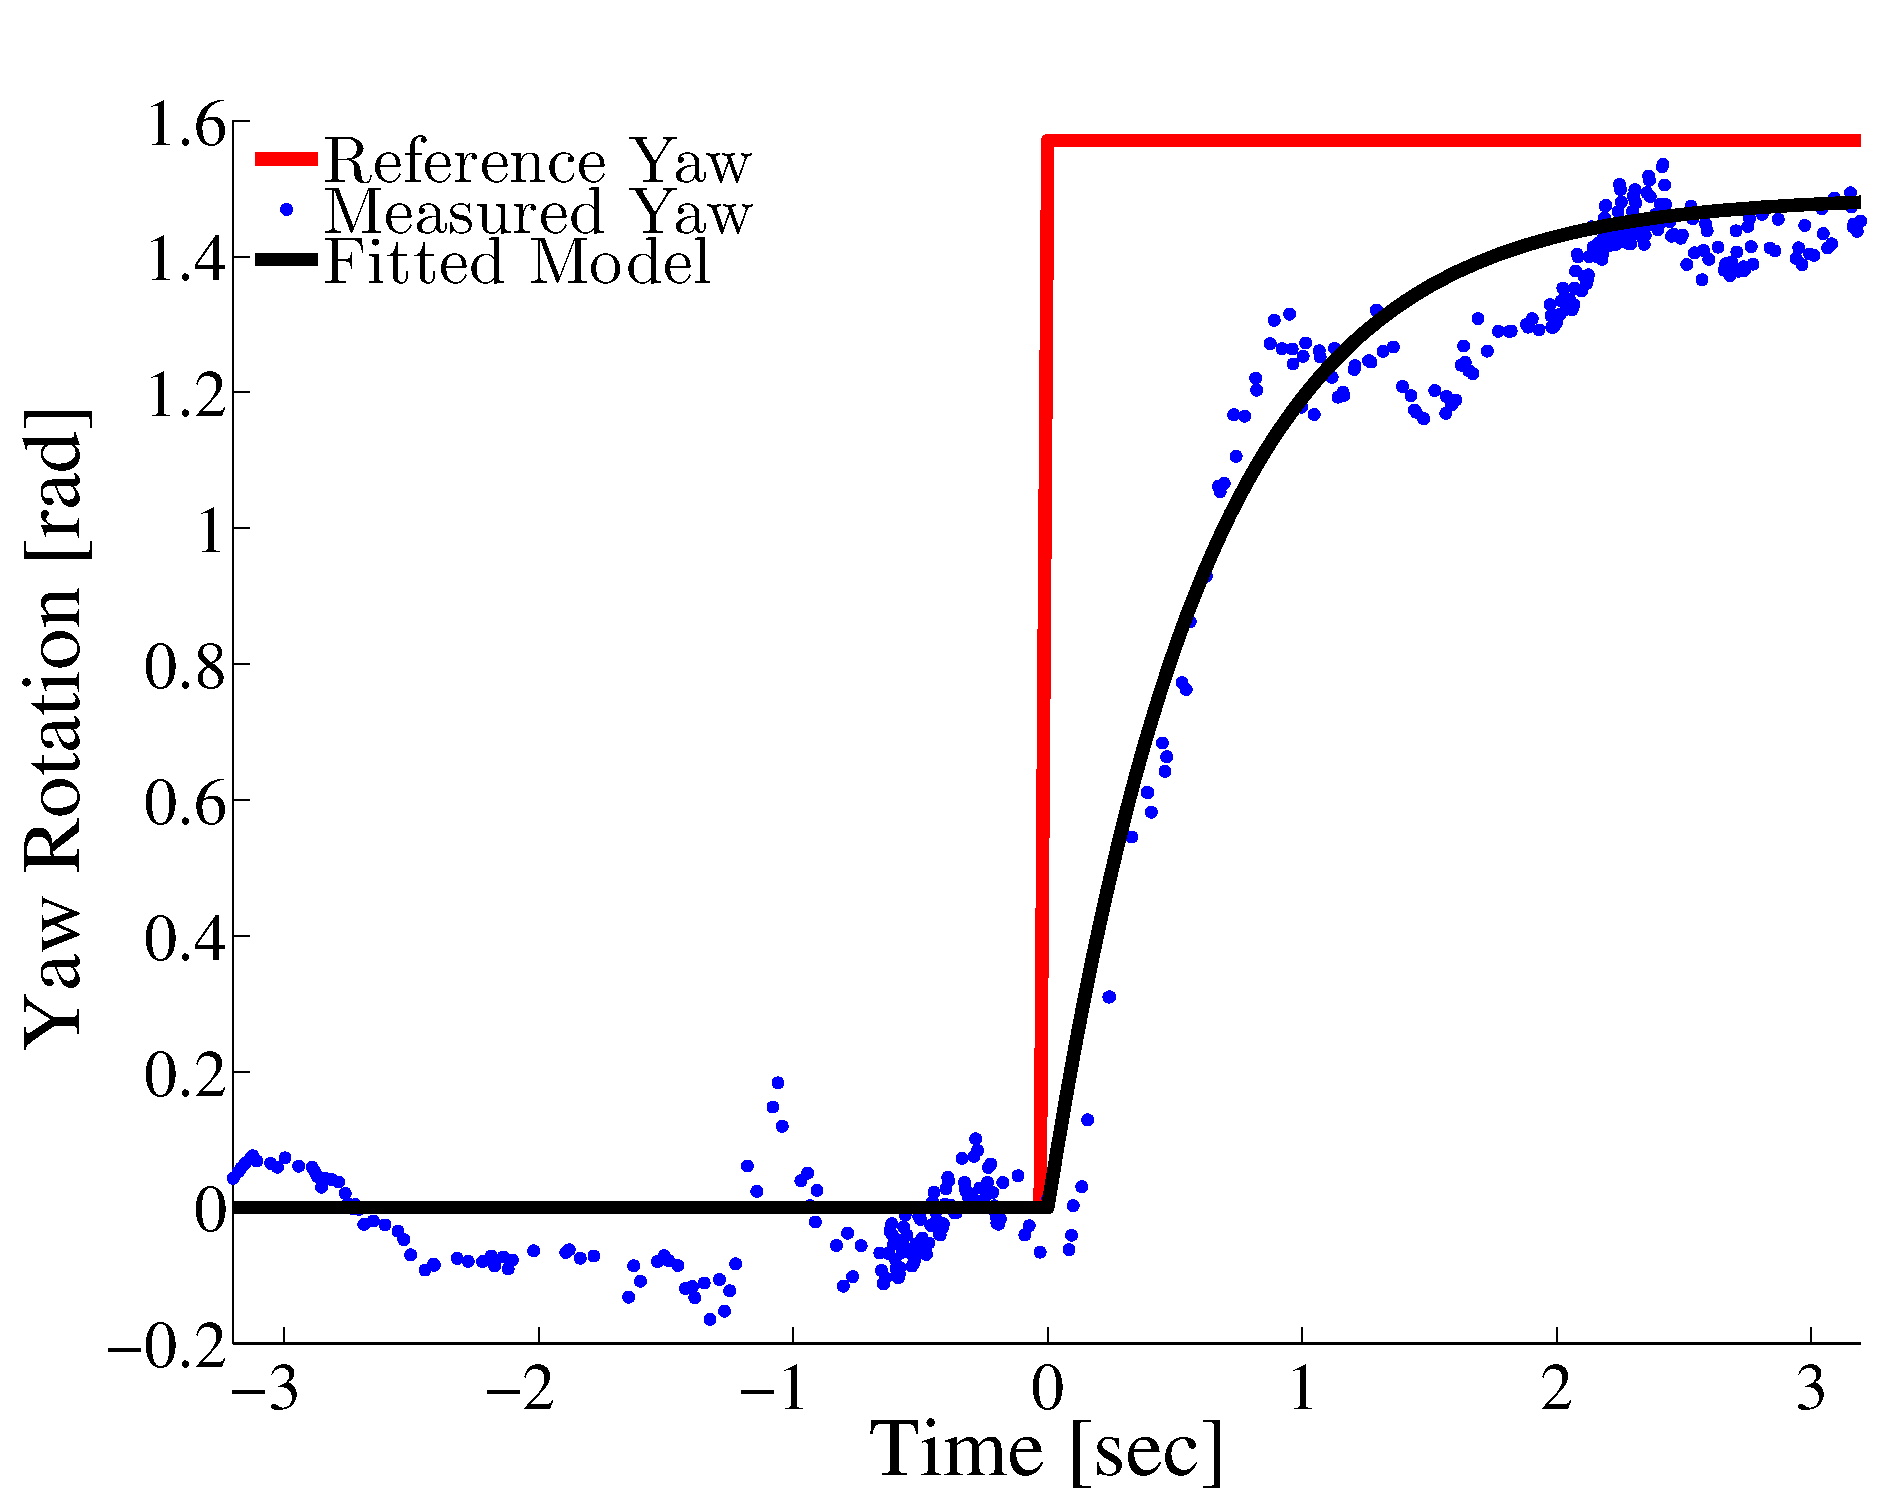
\includegraphics[width=\linewidth]{figures/step_response_total.pdf}
\caption{H$^2$Bird step response}
\label{fig:step_response}
\end{figure}
%TODO reduce number of sig figs

The first-order model that we fit to the step response of the onrithopter 
yaw motion is in Equation~\ref{eq:transfer_func}. This model represents the 
tuning dynamics of the ornithopter as well as the PID controller providing 
inputs to the actuators. We present the results of the the step response 
experiment, along with the response of the fitted model, in 
Figure~\ref{fig:step_response}.
\begin{equation}
\label{eq:transfer_func}
H(s) = \frac{0.95}{1+0.62s}
\end{equation}
The step response rise time is 1.4 seconds. The H$^2$Bird flies at an 
average forward velocity of 1.2 m/s during our experiments, so we estimate 
the minimum turning radius of the robot is 1.07 meters, as described in 
Equation~\ref{eq:min_radius}.
\begin{equation}
\label{eq:min_radius}
\begin{aligned}
\text{Minimum radius} & = \frac{360^{\circ}\times\text{Rise time}\times\text{Flight
speed}}{\text{Final angle}\times 2\pi}\\
& = \frac{360^{\circ}\times 1.4s\times 1.2\frac{m}{s}}{90^{\circ}\times2*\pi} = 1.07 m
\end{aligned}
\end{equation}
In the experiments we present in this work, we choose a flight speed lower 
than the maximum speed of the ornithopter, to facilitate more robust 
tracking.

%............................................................................%
\subsubsection{Ground Station Pose Estimation}

We measured a camera capture latency 40 ms, pose estimation computation 
latency of 12.5 ms, and radio latency of 25 ms.

%............................................................................%
\subsubsection{Cooperative Visual Servoing}
\label{sec:visual_servoing}

\begin{figure*}[tb]
\begin{minipage}[b]{0.45\linewidth}
\centering
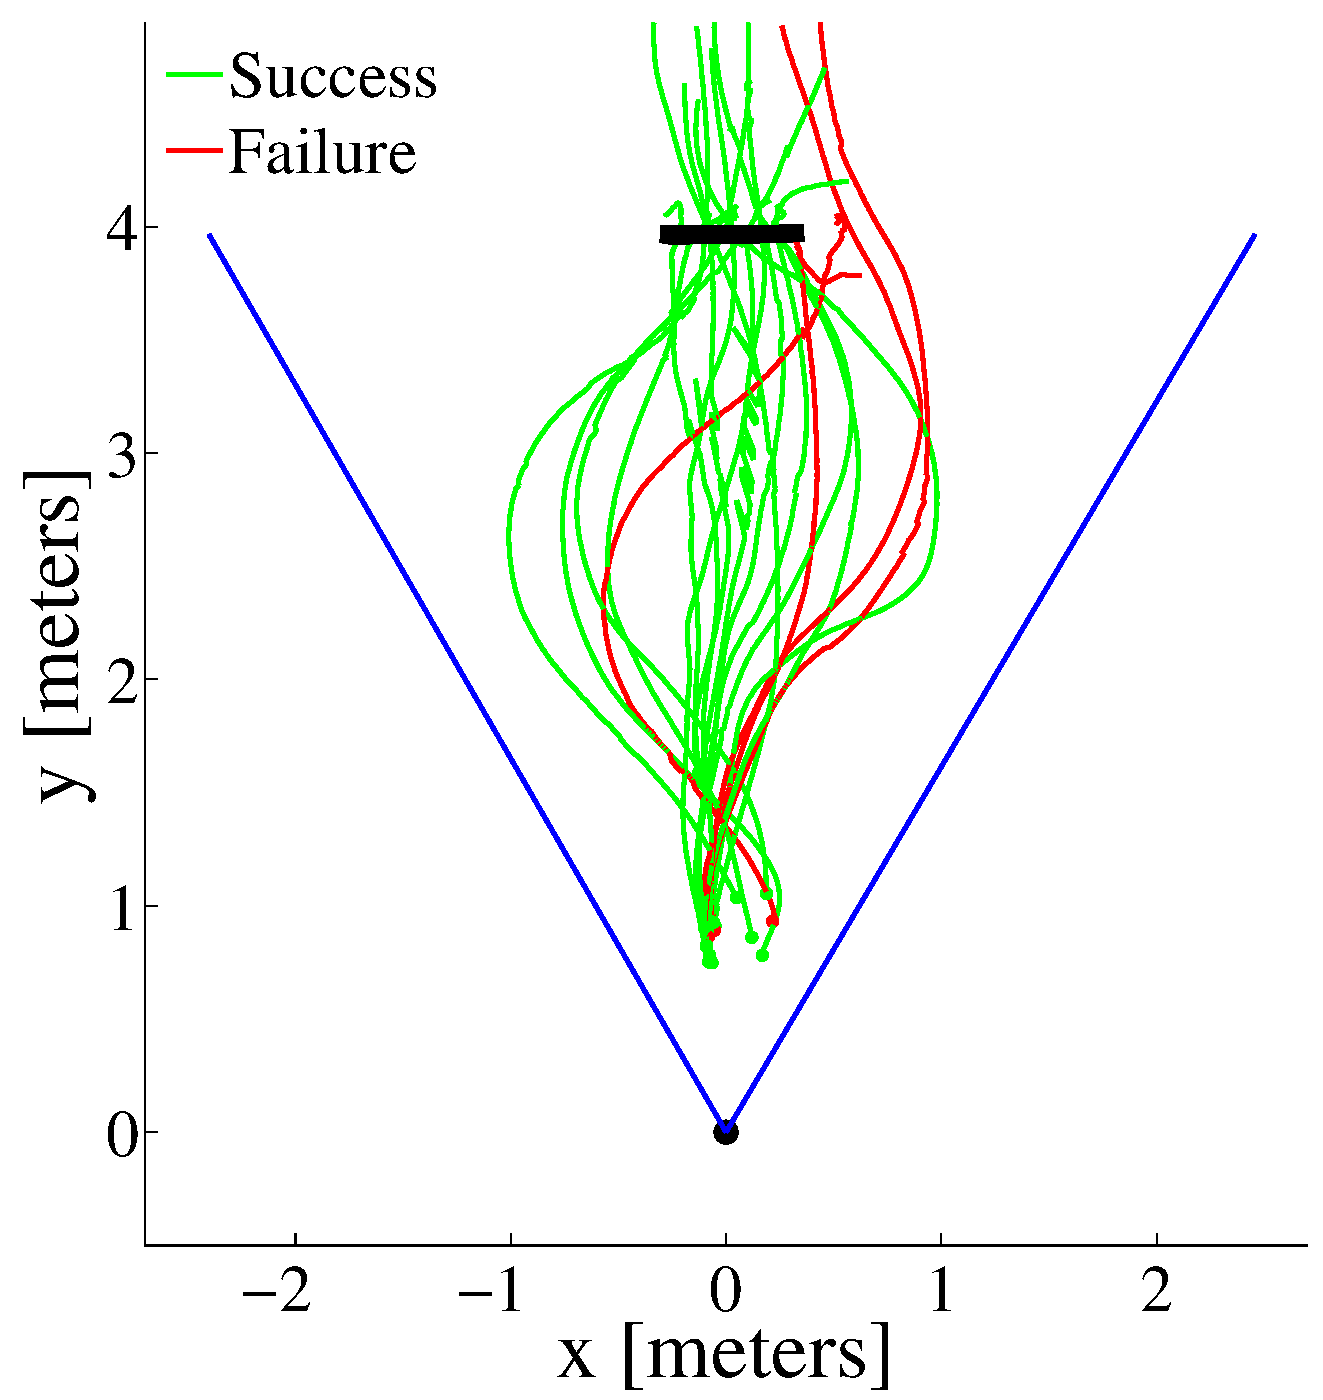
\includegraphics[width=\linewidth]{figures/flight_paths_feasible.pdf}
\caption{Plot of camera field of view and experimental trials within the feasible region.}
\label{fig:flight_paths_feasible}
\end{minipage}
\hfill
\begin{minipage}[b]{0.45\linewidth}
\centering
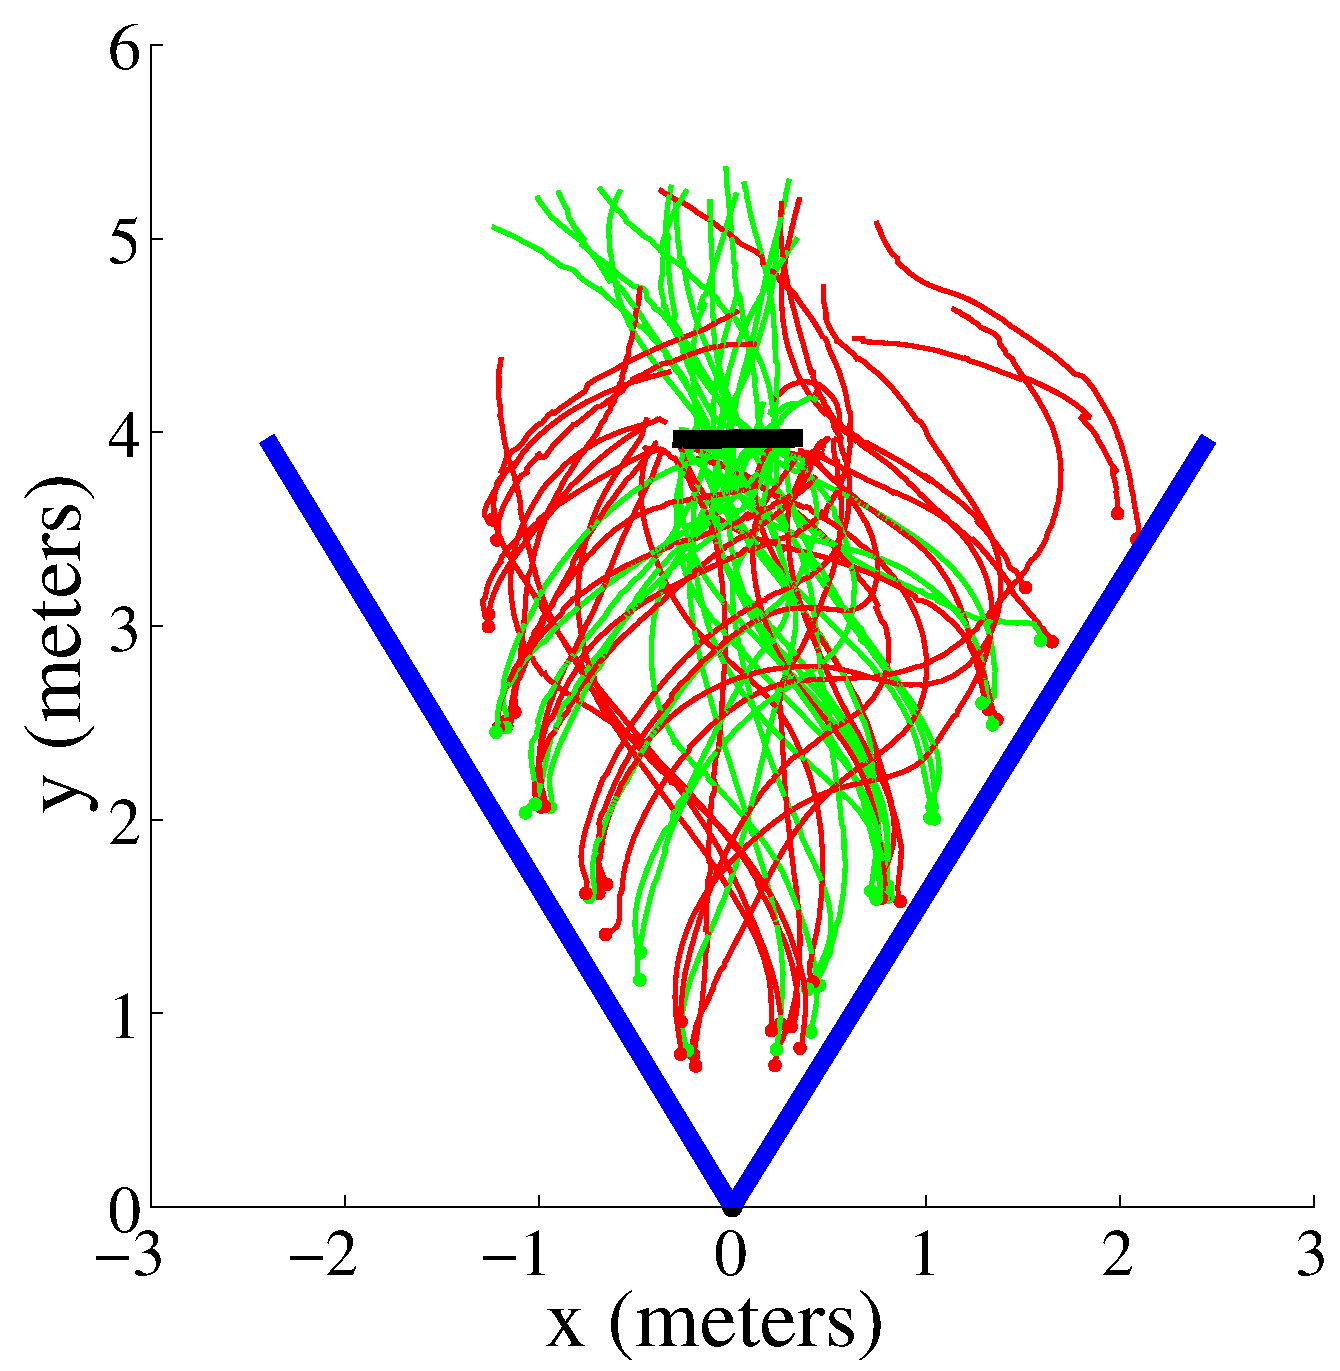
\includegraphics[width=\textwidth]{figures/flight_paths.pdf}
\caption{Plot of camera field-of-view and perimeter experimental trials overlayed.}
\label{fig:flight_paths}
\end{minipage}
\end{figure*}

Conducting the experimental trials as described in 
Section~\ref{sec:experiments_verification}, we achieved a success rate of 
80\% for initial conditions in the middle of the testing space and in front 
of the camera. As we moved towards the edges of the feasible region in 
Figure~\ref{fig:flight_paths}, the success rate diminished to 50\%. We 
present the results of our experimental trials in Figures~\ref{fig:flight_paths} 
and~\ref{fig:flight_paths_feasible}.

The lower success rate on the edges of the camera frame is explained by 
several factors. On the edges of the viewing triangle, the yaw control 
inputs are large in magnitude, although this is not necessary in all cases. 
Since the control algorithm we are using has no notion of depth, it applies 
the same control input whether the ornithopter is close to the camera, where 
small changes in heading are adequate, or far away from the camera, where 
large changes in heading are necessary. Due to this phenomenon, the 
controller often over or under-compensates in certain regions, depending 
upon the PID tuning and the distance from the camera. Tracking noise can 
also cause passage negotiation to fail. Variations in the H$^2$Bird hand 
launch can cause the system to respond differently for similar initial 
conditions. In addition, we changed H$^2$Bird battery approximately every 5 
tests, adding more variation to the H$^2$Bird performance by affecting the 
motor power output.

%----------------------------------------------------------------------------%
\subsection{Model Verification}

\begin{figure*}[tb]
\begin{minipage}[b]{0.45\linewidth}
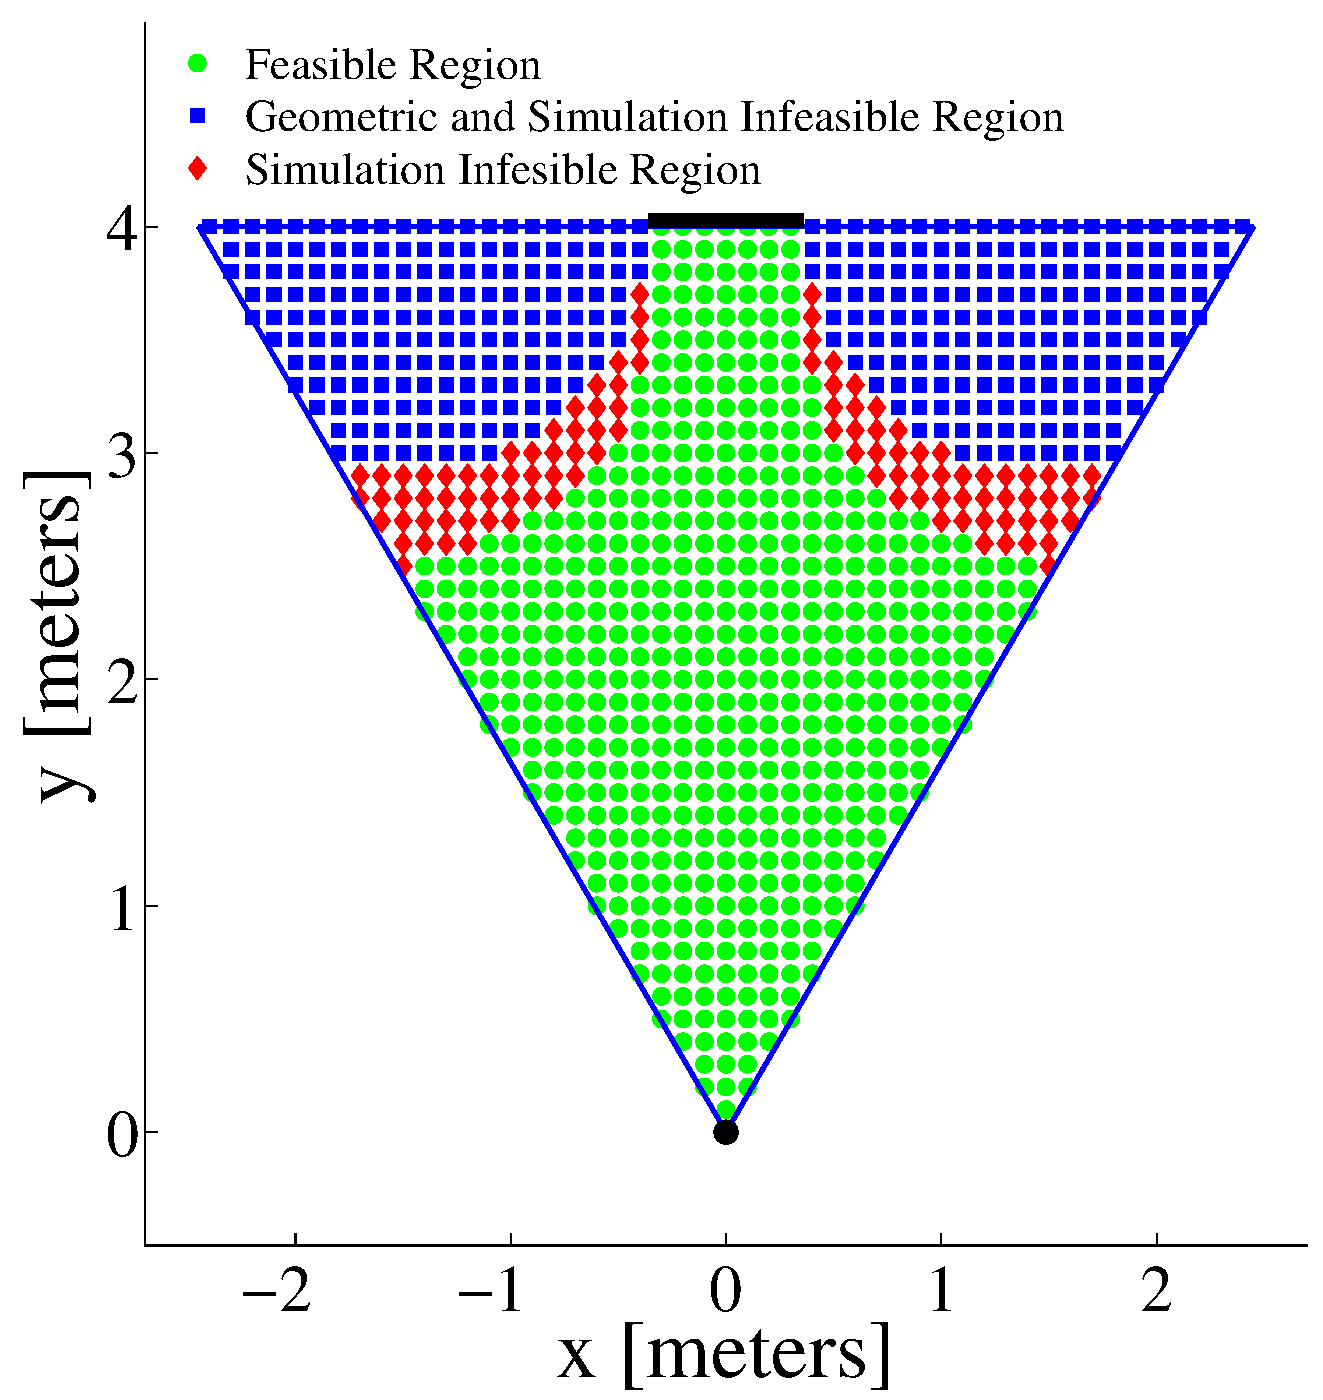
\includegraphics[width=\textwidth]{figures/feasible_set.pdf}
\caption{Plot of backwards reachable set for successful window traversal.}
\label{fig:feasible_set}
\end{minipage}
\hfill
\begin{minipage}[b]{0.45\linewidth}
\centering
\centering
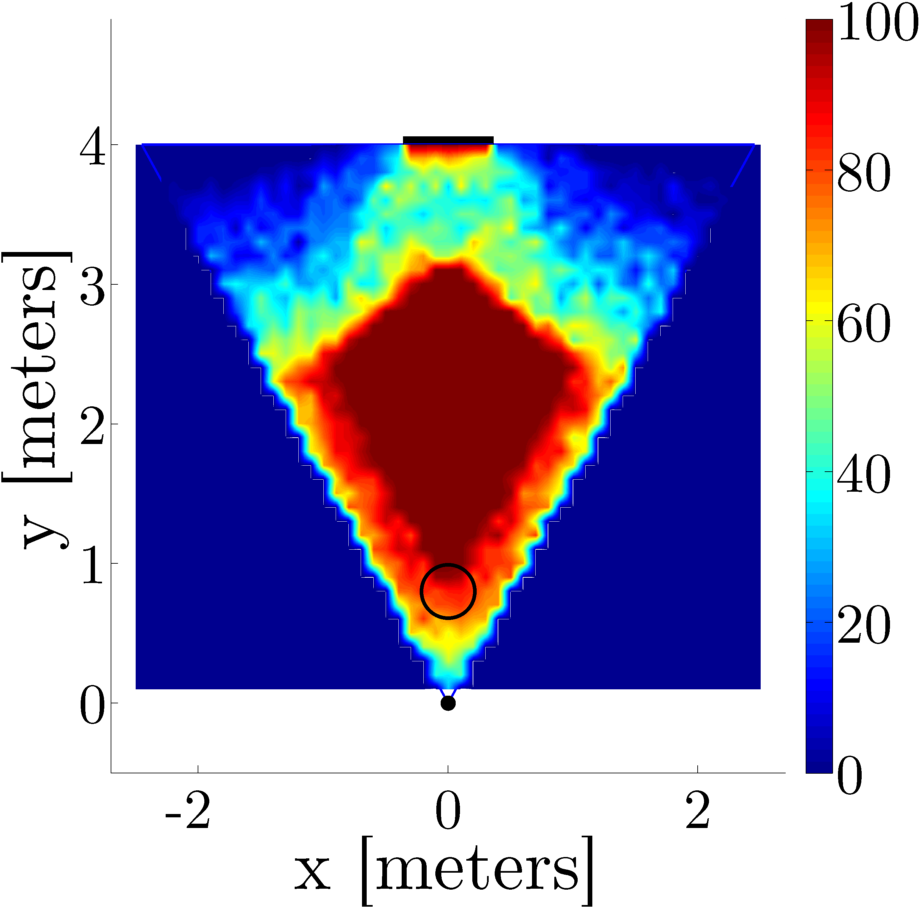
\includegraphics[width=\textwidth]{figures/heat_map.png}
\caption{Probability of success for all starting locations. This graphic is 
a result of a Monte Carlo simulation of the reachable set model, in which the 
initial heading of the H$^2$Bird is chosen uniformly at random from $(-90^{\circ},90^{\circ})$.}
\label{fig:heat_map}
\end{minipage}
\end{figure*}

We simulate the motion of the ornithopter beginning from various positional 
and angular heading initial conditions. We use this model, as determined 
through system identification (Sec.~\ref{sec:system_model}) using the 
cooperative control method in Figure~\ref{fig:block_diagram}.

We determine the backwards reachable set of initial states for successful 
narrow passage traversal both geometrically and in simulation 
(Fig.~\ref{fig:feasible_set}). In the figure, the blue lines represent the 
camera viewing triangle, the black line represents the window, and the black 
dot represents the camera. For the initial conditions, we used a uniform
grid of 5 cm increments within the camera viewing region, and an initial
angular heading perpendicular to the window plane. A success, or feasible 
initial condition, consists of a path that intersects the window at some 
point and does not leave the camera viewing triangle, and is indicated in 
green. The geometrically infeasible region is computed using the minimum 
turning radius and the geometry of the camera's field-of-view and is 
indicated in blue. The region in red is not geometrically feasible, but is 
infeasible as a result of the cooperative control simulation dynamics.

Our experimental data validates Figure~\ref{fig:feasible_set}, as there are 
no successes within the geometrically infeasible region. There are a few 
successes near the boundary of the infeasible region determined in 
simulation. While there are successes along the boundary of the camera 
viewing triangle, there are also many failures. We further explore this 
behavior using Monte Carlo simulation.

We conducted a Monte Carlo simulation to determine the probability of 
successful window navigation for a given point within the testing area. 
Using this information we can make assumptions about ideal starting 
positions for coopertive control. For each point within a 10 cm grid within 
the camera viewing triangle, we simulated 40 trials using an initial heading 
randomly sampled from a uniform distribution between -90$^{\circ}$ and 
90$^{\circ}$. Figure~\ref{fig:heat_map} depicts the results of the Monte 
Carlo simulation.

As shown in the figure, there is a region in the middle with a 100\% 
probability of success, which is a subset of the feasible region presented 
in Figure~\ref{fig:feasible_set}. Along the edges of the camera viewing 
triangle, however, the probability of success decreases.

The results of our experimental trials verify the results of the Monte Carlo
simulation of our model. The trials that we conducted in
Figure~\ref{fig:flight_paths_feasible} correspond to the circled region in
Figure~\ref{fig:heat_map}. The 80\% success rate that we measured in the
experiments corroborates our calculated probability of success of
approximately 80\%. Additionally, the diminished success rate of 50\% near the
edges of the viewing triangle that we determined through experimentation
supports the reduced probability of success calculated by the simulation.

%%%%%%%%%%%%%%%%%%%%%%%%%%%%%%%%%%%%%%%%%%%%%%%%%%%%%%%%%%%%%%%%%%%%%%%%%%%%%%
\section{Conclusions and Future Work}
We have demonstrated cooperative guidance of a 13 gram flapping-wing MAV with a
lightweight base station in hardware. In addition, we developed a model of the
cooperative system using system identification methods on the individual system capabilities, and composing
it with known system interactions. The corroboration between our simulated and
experimental results shows that our simplified modeling approach is useful for 
predicting the performance of cooperative systems at low computational cost. Our model could also be used to determine when to begin control with high probability of success, even though we lack information about the complete pose of the MAV.

We intend to further explore the benefits and limitations of collaboration in
unstructured environments by deploying our base station on millirobotic ground
vehicles. As the ground station used in this work was designed with this goal
in mind, this is a matter of implementation. The effectiveness of our modeling
approach, when applied to more complex systems with more interactions and 
agents is also a future area of interest. 

%%%%%%%%%%%%%%%%%%%%%%%%%%%%%%%%%%%%%%%%%%%%%%%%%%%%%%%%%%%%%%%%%%%%%%%%%%%%%%
\section{Acknowledgments}
The authors would like to thank Fernando Garcia Bermudez for his 
assistance with the Vicon motion capture system, Andrew Pullin for his 
help with robot photography, and the members of the Biomimetic 
Millisystems Laboratory and the EECS community at the University of 
California, Berkeley for their advice and support.

%%%%%%%%%%%%%%%%%%%%%%%%%%%%%%%%%%%%%%%%%%%%%%%%%%%%%%%%%%%%%%%%%%%%%%%%%%%%%%%

%%%%%%%%%%%%%%%%%%%%%%%%%%%%%%%%%%%%%%%%%%%%%%%%%%%%%%%%%%%%%%%%%%%%%%%%%%%%%%%
% BIBLIOGRAPHY

% The following two commands are all you need in the
% initial runs of your .tex file to
% produce the bibliography for the citations in your paper.
\bibliographystyle{abbrv}
\bibliography{manuscript}

% ACM needs 'a single self-contained file'!
%\subsection{References}
% Generated by bibtex from your ~.bib file.  Run latex,
% then bibtex, then latex twice (to resolve references)
% to create the ~.bbl file.  Insert that ~.bbl file into
% the .tex source file and comment out
% the command \texttt{{\char'134}thebibliography}.
\end{document}
